% Options for packages loaded elsewhere
\PassOptionsToPackage{unicode}{hyperref}
\PassOptionsToPackage{hyphens}{url}
\PassOptionsToPackage{dvipsnames,svgnames,x11names}{xcolor}
%
\documentclass[
  letterpaper,
  DIV=11,
  numbers=noendperiod,
  oneside]{scrreprt}

\usepackage{amsmath,amssymb}
\usepackage{lmodern}
\usepackage{iftex}
\ifPDFTeX
  \usepackage[T1]{fontenc}
  \usepackage[utf8]{inputenc}
  \usepackage{textcomp} % provide euro and other symbols
\else % if luatex or xetex
  \usepackage{unicode-math}
  \defaultfontfeatures{Scale=MatchLowercase}
  \defaultfontfeatures[\rmfamily]{Ligatures=TeX,Scale=1}
\fi
% Use upquote if available, for straight quotes in verbatim environments
\IfFileExists{upquote.sty}{\usepackage{upquote}}{}
\IfFileExists{microtype.sty}{% use microtype if available
  \usepackage[]{microtype}
  \UseMicrotypeSet[protrusion]{basicmath} % disable protrusion for tt fonts
}{}
\makeatletter
\@ifundefined{KOMAClassName}{% if non-KOMA class
  \IfFileExists{parskip.sty}{%
    \usepackage{parskip}
  }{% else
    \setlength{\parindent}{0pt}
    \setlength{\parskip}{6pt plus 2pt minus 1pt}}
}{% if KOMA class
  \KOMAoptions{parskip=half}}
\makeatother
\usepackage{xcolor}
\usepackage[left=1in,marginparwidth=2.0666666666667in,textwidth=4.1333333333333in,marginparsep=0.3in]{geometry}
\setlength{\emergencystretch}{3em} % prevent overfull lines
\setcounter{secnumdepth}{5}
% Make \paragraph and \subparagraph free-standing
\ifx\paragraph\undefined\else
  \let\oldparagraph\paragraph
  \renewcommand{\paragraph}[1]{\oldparagraph{#1}\mbox{}}
\fi
\ifx\subparagraph\undefined\else
  \let\oldsubparagraph\subparagraph
  \renewcommand{\subparagraph}[1]{\oldsubparagraph{#1}\mbox{}}
\fi


\providecommand{\tightlist}{%
  \setlength{\itemsep}{0pt}\setlength{\parskip}{0pt}}\usepackage{longtable,booktabs,array}
\usepackage{calc} % for calculating minipage widths
% Correct order of tables after \paragraph or \subparagraph
\usepackage{etoolbox}
\makeatletter
\patchcmd\longtable{\par}{\if@noskipsec\mbox{}\fi\par}{}{}
\makeatother
% Allow footnotes in longtable head/foot
\IfFileExists{footnotehyper.sty}{\usepackage{footnotehyper}}{\usepackage{footnote}}
\makesavenoteenv{longtable}
\usepackage{graphicx}
\makeatletter
\def\maxwidth{\ifdim\Gin@nat@width>\linewidth\linewidth\else\Gin@nat@width\fi}
\def\maxheight{\ifdim\Gin@nat@height>\textheight\textheight\else\Gin@nat@height\fi}
\makeatother
% Scale images if necessary, so that they will not overflow the page
% margins by default, and it is still possible to overwrite the defaults
% using explicit options in \includegraphics[width, height, ...]{}
\setkeys{Gin}{width=\maxwidth,height=\maxheight,keepaspectratio}
% Set default figure placement to htbp
\makeatletter
\def\fps@figure{htbp}
\makeatother

\KOMAoption{captions}{tableheading}
\makeatletter
\makeatother
\makeatletter
\@ifpackageloaded{bookmark}{}{\usepackage{bookmark}}
\makeatother
\makeatletter
\@ifpackageloaded{caption}{}{\usepackage{caption}}
\AtBeginDocument{%
\ifdefined\contentsname
  \renewcommand*\contentsname{Table of contents}
\else
  \newcommand\contentsname{Table of contents}
\fi
\ifdefined\listfigurename
  \renewcommand*\listfigurename{List of Figures}
\else
  \newcommand\listfigurename{List of Figures}
\fi
\ifdefined\listtablename
  \renewcommand*\listtablename{List of Tables}
\else
  \newcommand\listtablename{List of Tables}
\fi
\ifdefined\figurename
  \renewcommand*\figurename{Figure}
\else
  \newcommand\figurename{Figure}
\fi
\ifdefined\tablename
  \renewcommand*\tablename{Table}
\else
  \newcommand\tablename{Table}
\fi
}
\@ifpackageloaded{float}{}{\usepackage{float}}
\floatstyle{ruled}
\@ifundefined{c@chapter}{\newfloat{codelisting}{h}{lop}}{\newfloat{codelisting}{h}{lop}[chapter]}
\floatname{codelisting}{Listing}
\newcommand*\listoflistings{\listof{codelisting}{List of Listings}}
\makeatother
\makeatletter
\@ifpackageloaded{caption}{}{\usepackage{caption}}
\@ifpackageloaded{subcaption}{}{\usepackage{subcaption}}
\makeatother
\makeatletter
\@ifpackageloaded{tcolorbox}{}{\usepackage[many]{tcolorbox}}
\makeatother
\makeatletter
\@ifundefined{shadecolor}{\definecolor{shadecolor}{rgb}{.97, .97, .97}}
\makeatother
\makeatletter
\@ifpackageloaded{sidenotes}{}{\usepackage{sidenotes}}
\@ifpackageloaded{marginnote}{}{\usepackage{marginnote}}
\makeatother
\makeatletter
\makeatother
\ifLuaTeX
  \usepackage{selnolig}  % disable illegal ligatures
\fi
\IfFileExists{bookmark.sty}{\usepackage{bookmark}}{\usepackage{hyperref}}
\IfFileExists{xurl.sty}{\usepackage{xurl}}{} % add URL line breaks if available
\urlstyle{same} % disable monospaced font for URLs
\hypersetup{
  pdftitle={Lexical Portraits},
  pdfauthor={Ligeia Lugli},
  colorlinks=true,
  linkcolor={blue},
  filecolor={Maroon},
  citecolor={Blue},
  urlcolor={Blue},
  pdfcreator={LaTeX via pandoc}}

\title{Lexical Portraits}
\usepackage{etoolbox}
\makeatletter
\providecommand{\subtitle}[1]{% add subtitle to \maketitle
  \apptocmd{\@title}{\par {\large #1 \par}}{}{}
}
\makeatother
\subtitle{Part of A Visual Dictionary and Thesaurus of Buddhist
Sanskrit}
\author{Ligeia Lugli}
\date{31/03/2022}

\begin{document}
\maketitle
\ifdefined\Shaded\renewenvironment{Shaded}{\begin{tcolorbox}[frame hidden, interior hidden, borderline west={3pt}{0pt}{shadecolor}, enhanced, sharp corners, breakable, boxrule=0pt]}{\end{tcolorbox}}\fi

\renewcommand*\contentsname{Table of contents}
{
\hypersetup{linkcolor=}
\setcounter{tocdepth}{2}
\tableofcontents
}
\bookmarksetup{startatroot}

\hypertarget{preface}{%
\chapter{Preface}\label{preface}}

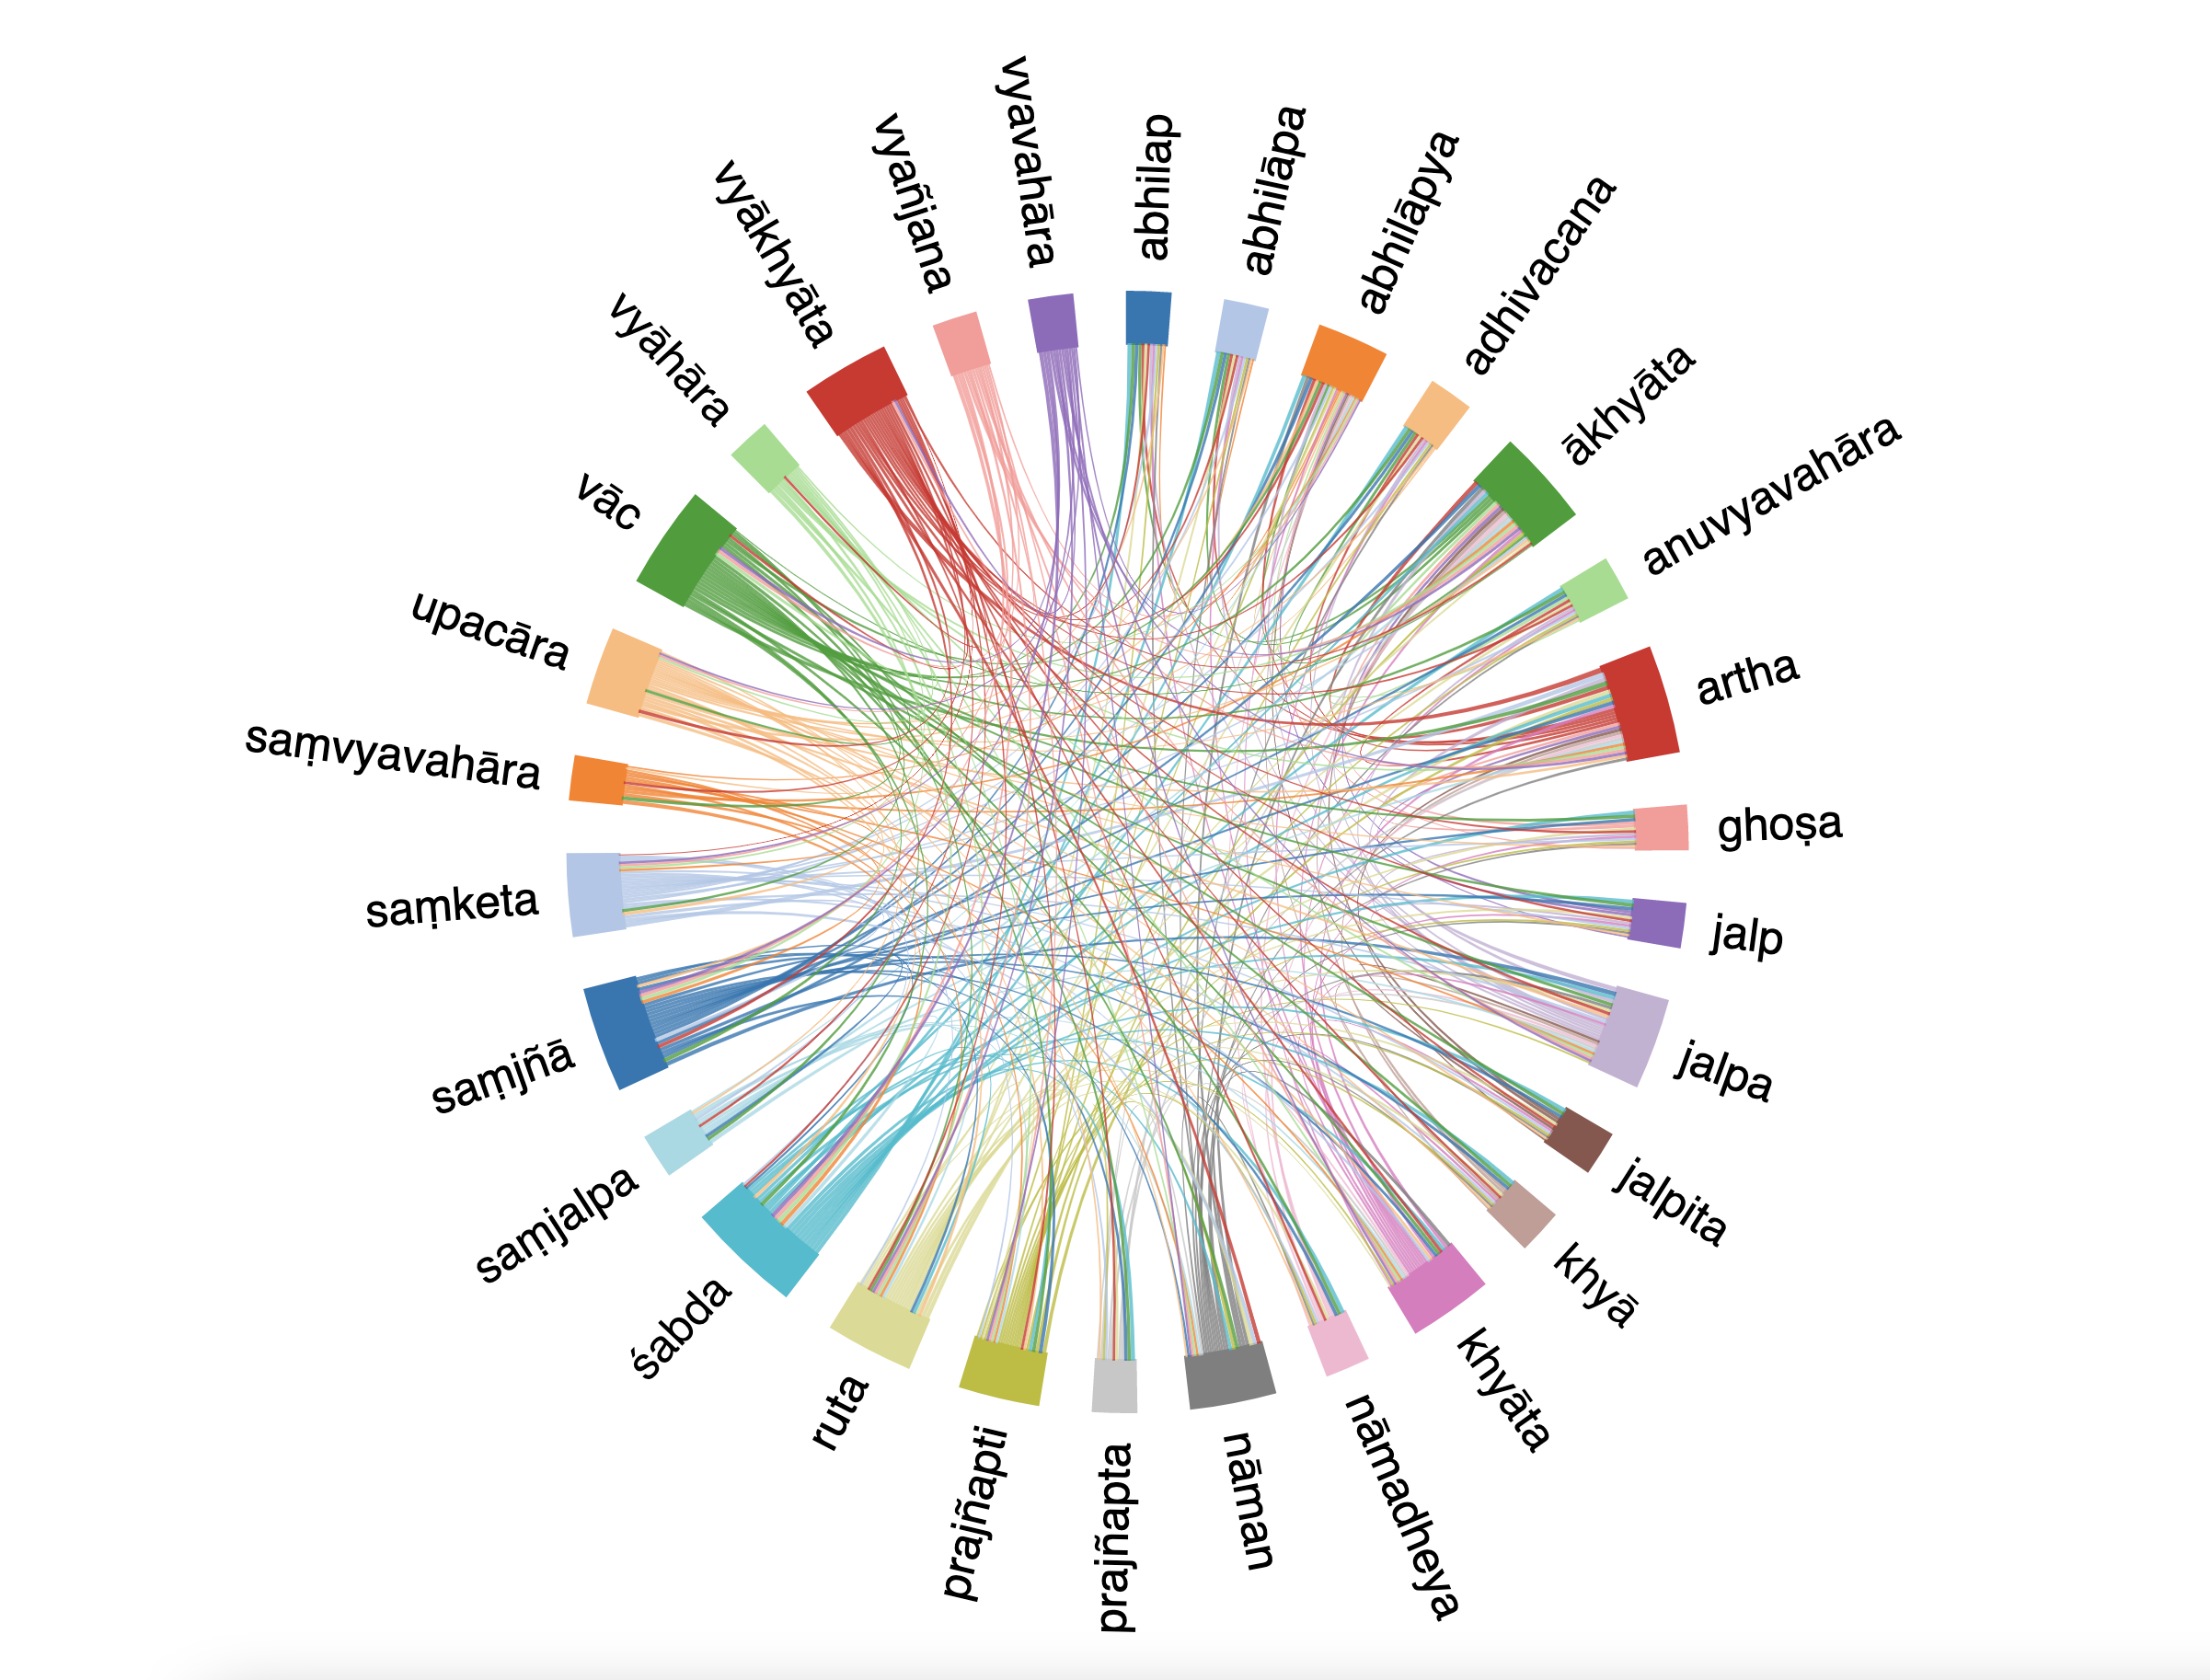
\includegraphics{./SynchordLanguage.png}

\texttt{Lexical\ Portraits} is a series of in-depth analyses of core
Buddhist Sanskrit vocabulary launched by the Buddhist Translators
Workbench in 2021, as part of the lexicographic programme run by the
Mangalam Research Center.

Each portrait is meant to be perused in conjunction with the
corresponding entry in the Visual Dictionary and Thesaurus of Buddhist
Sanskrit. While the dictionary entries allow interactive exploration of
our manually annotated citations, the portraits offer our own
interpretation of those citation as well as of corpus data. Contrary to
the dictionary, where all charts are automated, the Portraits'
data-visualizations are manually tailored to each lemma. We recommend to
always check the \texttt{info} tabs that accompany the portraits'
graphs, as the statistics and principles used to generate the graphs may
vary from headword to headword.

More information about the editorial strategy and theoretical
underpinnings of the Lexical Portraits series can be found in Ligeia
Lugli (2021) Dictionaries as Collections of Lexical Data Stories: an
alternative post-editing model for historical lexicography. eLex 2021
proceedings.

\hypertarget{coverage}{%
\subsection{coverage}\label{coverage}}

The vocabulary we intend to cover in our Lexical Portrait is a subset of
the headwords we are going to cover in the Visual Dictionary and
Thesaurus of Buddhist Sanskrit. We prioritize words that are relatively
frequent in the corpus, are difficult to translate, and lexicalize
important concepts in Buddhism.

\hypertarget{corpus}{%
\subsection{corpus}\label{corpus}}

The Lexical Portraits are based on a \textasciitilde7 million words
corpus of Buddhist Sanskrit literature that we are currently expanding
thanks to funding from the Khyentse Foundation.

The corpus is available on Zenodo; the \texttt{info} tabs of each
portrait detail which version of the corpus has been used for a
particular portrait.

Graphs and information based on manual annotations draw on the subset of
the corpus that is used for our dictionary. Please refer to the
\texttt{Corpus} section of the Visual Dictionary and Thesaurus of
Buddhist Sanskrit for a list of the texts included on the subcorpus we
use for manual annotation.

\hypertarget{team}{%
\subsection{team}\label{team}}

The Lexical Portraits are created by Ligeia Lugli on the basis of
linguistic annotations by Luis Gamaliel Quiñones Martinez.

\bookmarksetup{startatroot}

\hypertarget{prajuxf1apti}{%
\chapter{prajñapti}\label{prajuxf1apti}}

{\marginnote{\begin{footnotesize}\emph{kiṃ c\^{}edaṃ dravyata iti kiṃ vā
\textbf{prajñapt}itaḥ / rūp\^{}ādivat bhāv\^{}āntaraṃ cet dravyataḥ /
kṣīr\^{}ādivat samudāyaś cet prajñaptitaḥ /} {[}abhidharmakośabhāṣya,
461{]}\\
``Does the pudgala exists as a real entity or as a nominal construct? If
a person is a distinct entity like visible form and other such things,
he is substantially real; but if {[}by analysis{]} he is {[}shown to
be{]} a collection {[}of substances{]}, like milk and other such things,
he is real by way of a conception.'' {[}Duerlinger
73{]}\end{footnotesize}}}

The core meaning of prajñapti (also spelled prajñāpti) is close to its
etymological sense, which conveys the idea of `making known'. In our
corpus, this broad sense finds two main semantic applications, the
closely related meaning of verbal expression and the derived sense of
designating something for a specific use (designating for a
use/allocating), which typically refers to allocating seats to
participants in an assembly (e.g Divyāvadāna, 468.017). \footnote{\emph{bahir
  nagarasya pañca vihāra-śatāni kāritāni pañca
  mañca-pīṭha-vṛṣi-koccaka-bimbopadhāna-caturasraka-śatāni dāpitāni
  pañca piṇḍapāta-śatāni prajñaptāni vistīrṇ\^{}-āvakāśe ca
  pṛthivī-pradeśe āsana-\textbf{prajñaptiḥ}} \emph{kāritā
  /}{[}divyāvadāna\_selection, 468.017{]}\\
  ``He also commissioned five hundred monastic dwellings outside of the
  city; gave out five hundred chairs, seats, cushions, woolen blankets,
  pillows, and shawls; distributed five hundred meals; and had a seat
  specially prepared for the venerable Mahākātyāyana in a wide-open
  tract of land.'' {[}Rotman{]}}

The former sense is by far the most widespread and semantically nuanced.
It comprises several different uses, all of which stand on continuum
between verbal expressions and their cognitive counterpart, that is,
concepts and notions, e.g.~Abhidharmakośabhāṣya, 140. \footnote{\emph{yath\^{}oktam
  ātmā ātm\^{}eti bhikṣavo bālo 'śrutavān pṛthagjanaḥ
  \textbf{prajñapt}im anupatito na tv atr\^{}ātmā vā ātmīyaṃ vā iti /}
  {[}abhidharmakośabhāṣya, 140{]}\\
  ``It is said in fact, `The fool, the ignorant, the Pṛthagjana,
  conforming to the manners of vulgar speech, thinks ``me,'' or
  ``mine;'' but there is not any ``me'' or ``mine.''\,'\,'' {[}Pruden
  419{]}}

This latter use (labelled verbal expression/notion), finds a specialized
application in the Buddhist ontological discourse, especially (but not
exclusively) in abhidharmic contexts, where it comes to denote the
merely conceptual nature of phenomena ,or nominal existence (+sat). In
this sense, prajñapti is typically compounded with sat and contrasted
with dravya-sat, e.g.~Abhisamayālaṃkāra, 5.5. \footnote{\emph{dravya-\textbf{prajñapti}-sat-sattva-vikalpau
  grāhakau matau / pṛthagjan\^{}-ārya-bhedena pratyekaṃ tau
  nav\^{}-ātmakau // 5.6 //} {[}abhisamayālaṃkāra, 5.5{]}\\
  ``(The Sutra then) considers the two (false) discriminations of the
  subject. The one regards beings (or persons) as (real) substantial
  entities, the second as (merely) nominal entities. The first refers to
  the common people, the second to the saints. Each one consists of nine
  items.'' {[}Conze 81{]}}

In contrast to this specialized meaning, the sense of prajñapti as
verbal expression is much broader. It encompasses one-word designations
(e.g.~Mahāvastu, 1.351) \footnote{\emph{teṣāṃ dāni kumārāṇāṃ śakyaṃ
  śākiyā ti samākhyā-samājñā-\textbf{prajñapti}udapāsi //} {[}mahāvastu,
  1.351{]}\\
  ``\,`Cunning, sirs, are these princes.' And from the `cunning' of
  these princes arose their name, appellation and designation of
  Śākiyans.'' {[}Jones 297{]}} as well as statements and lengthy
expositions, such as the exposition/formulation of teachings and
monastic rules (e.g.~Bhikṣuṇīvinaya, 179). \footnote{\emph{\ldots{} iti
  svayan na upasampādayet niḥsargika-pācattikaṃ / yāvat
  \textbf{prajñaptiḥ}/} {[}bhikṣuṇīvinaya, 179{]}\\
  ``C'est une faute entraînant abandon {[}de l'objet en cause{]} et aveu
  formel -etc \ldots{} promulgation.'' {[}Nolot 178{]}} In this sense,
prajñapti features in the title of several works and in our corpus it
appears to refer to the title of a treatise in particular,
e.g.~Abhidharmakośabhāṣya, 419) \footnote{\emph{\textbf{prajñapt}au tu
  pratisaṃvidām eva nirdeśaḥ /} {[}abhidharmakośabhāṣya, 419{]}\\
  ``According to the Prajñaptipāda, the Unhindered Knowledges are in the
  following order: {[}\ldots{]}.'' {[}Pruden 1154{]}}

The boundaries between these uses of prajñapti tend to be blurry. The
semantic categorization we provide is, at best, porous, as it is often
impossible to determine whether in a given passage this word refers to a
designation, a notion or an entity that is only taken to exist
nominally.

\begin{figure}

{\centering 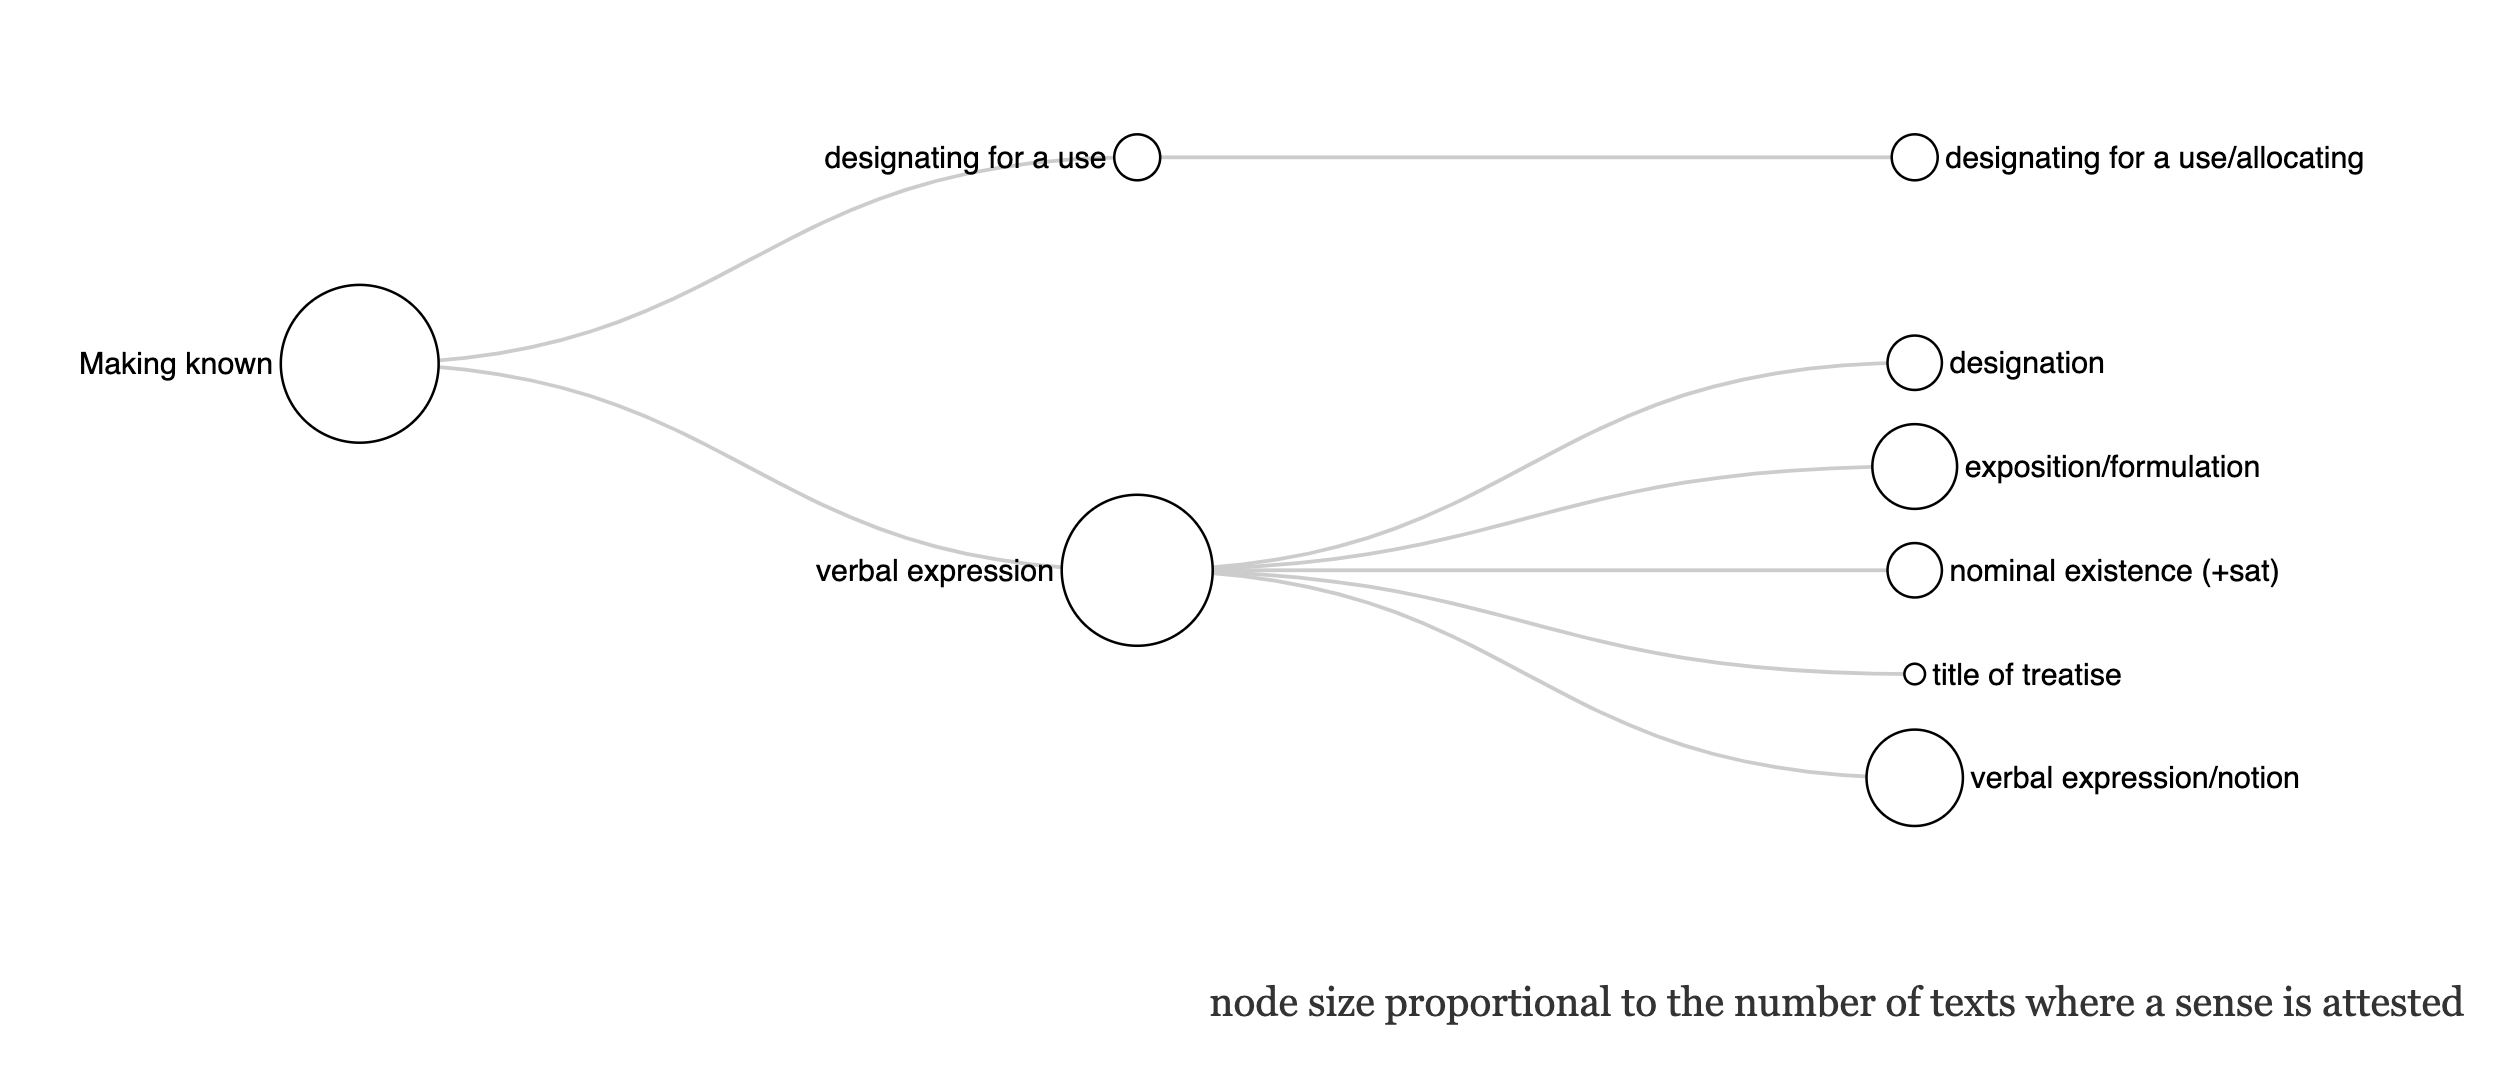
\includegraphics{./www/semanticTree_prajJapti.png}

}

\caption{\label{fig-semantictree}semantic tree}

\end{figure}

\hypertarget{sec-freq}{%
\section{frequency}\label{sec-freq}}

prajñapti is a mid-frequency word in our corpus (see frequency graph
below). While its dispersion over genres is relatively even when
compared to other words in our corpus (see graphs on the right),

\begin{marginfigure}

{\centering \includegraphics{./www/genreDP_prajJapti.webp}

}

\caption{\label{fig-genredp}genre dispersion}

\end{marginfigure}

the graph in the next section shows that prajñapti is in fact mostly
attested in vinaya, sūtra and śāstra literature; whereas it is extremely
rare in other genres.

An analysis of the the distribution of its senses reveals further
differences in the use of prajñapti across genres (see sense by genre
tab).

The sense of exposition/formulation, which is perhaps the closest to the
core meaning of the headword, is the only one to be attested in all
genres. By contrast, the sense of verbal expression/notion, which is
responsible for most attestations of prajñapti in the sample of
sentences that we have manually annotated for the dictionary, is limited
to śāstra and sūtra material.

Prajñapti's dispersion over periods is very similar to its dispersion
over genres; but it is more in line with the diachronic dispersion of
other words in our corpus, which tend to be more evenly dispersed across
periods than across genres (see genre dispersion graph on the right).

\begin{marginfigure}

{\centering \includegraphics{./www/periodDP_prajJapti.webp}

}

\caption{\label{fig-perioddp}period dispersion}

\end{marginfigure}

Nevertheless, prajñapti's normalised frequency drops noticeably in the
later `commentarial' layer of the corpus, which dates from the VI
century onwards (see frequency by period tab).

\hypertarget{sec-freqcurve}{%
\subsubsection{frequency graph}\label{sec-freqcurve}}

\marginnote{\begin{footnotesize}

Frequency and dispersion are calculated over the
\textasciitilde7-million words Segmented Corpus of Buddhist Sanskrit
(10.5281/zenodo.3457822).

Dispersion is calculated with Gries' deviation of proportion formula
(Gries, S. 2008. Dispersion and adjusted frquencies in corpora.
International Journal of Corpus Linguistics, 13(4): 403-437)

\end{footnotesize}}

\begin{figure}

{\centering \includegraphics{./www/ZipfCurveFreq_prajJapti.webp}

}

\caption{\label{fig-freq}lemma's frequency compared to near-synonyms}

\end{figure}

\hypertarget{sec-sensebygenre}{%
\subsubsection{sense by genre}\label{sec-sensebygenre}}

\begin{figure*}

{\centering 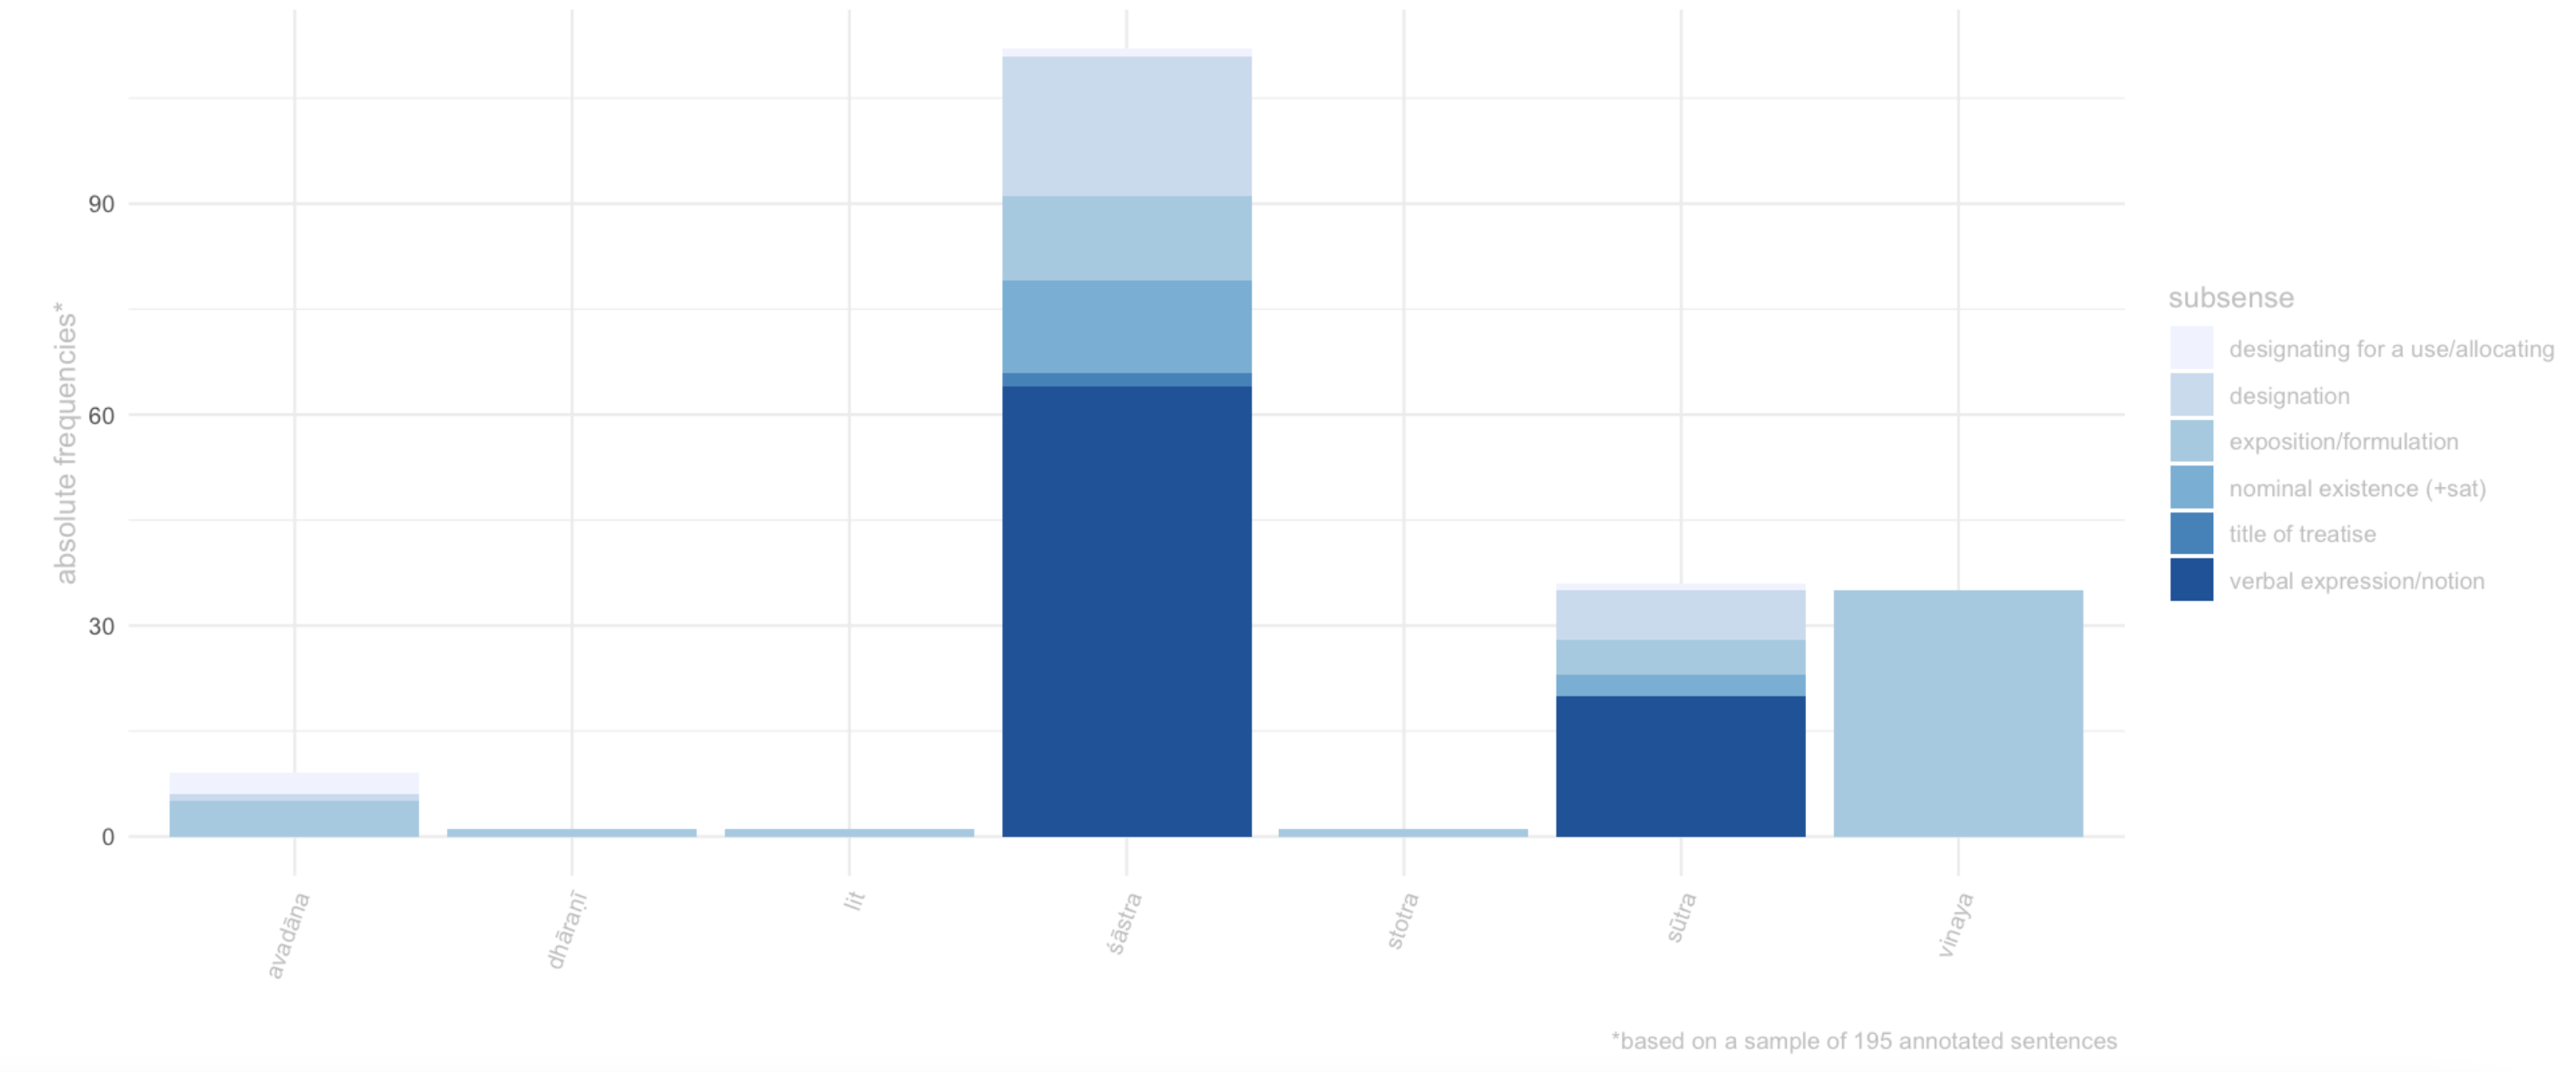
\includegraphics{./www/SenseByGenre_prajJapti.png}

}

\caption{\label{fig-sensebygenre}sense by genre}

\end{figure*}

\hypertarget{sec-freqbyperiod}{%
\subsubsection{frequency by period}\label{sec-freqbyperiod}}

\begin{figure}

{\centering \includegraphics{./www/PeriodFreq_prajJapti.webp}

}

\caption{\label{fig-freqbyperiod}frequency by period}

\end{figure}

\hypertarget{sec-disperioninfo}{%
\subsubsection{info}\label{sec-disperioninfo}}

frequency and dispersion are calculated over the
\textasciitilde7-million words Segmented Corpus of Buddhist Sanskrit
(10.5281/zenodo.3457822), as opposed to the smaller corpus used for the
Visual Dictionary and Thesaurus of Buddhist Sanskrit (see dictionary
documentation for details).

For the sake of readability, only words occurring at least 5 times in
the corpus have been plotted on the frequency and dispersion curves.

Dispersion is calculated with Gries' deviation of proportion formula
(Gries, S. 2008. Dispersion and adjusted frquencies in corpora.
International Journal of Corpus Linguistics, 13(4): 403-437).

the sense by genre plot is based on a sample of sentences that we have
manually annotated with semantic information for the Visual Dictionary
and Thesaurus of Buddhist Sanskrit. For details about our sampling and
annotation procedures see the dictionary documentation page.

\hypertarget{sec-register}{%
\section{register}\label{sec-register}}

register Overall, the distribution of prajñapti over the genres points
to a rather formal register and a predominantly scholastic use. Even the
sense of designating something for use, which recurs in storytelling
settings, appears to be crystallized in a formula and lack the
contextual malleability of general-language words. The meaning of
exposition/application, too, has a formulaic flavor in the Vinaya (see
examples from the Bhikṣuṇivanaya) where it denotes the codification of
rules, a meaning that emerges also in other genres, where prajñapti
expresses a sense close to the English `precepts'
(e.g.~Bodhicāryāvatara, 2.63). Finally, the specialized use of prajñapti
+ sat has terminological value, as it corresponds to a specific node in
the Buddhist ontological system. Uses of this word without sat in
Mahāyāna homiletic contexts, such as in statements to the effect that
all is `mere prajñapti' (e.g.~Laṅkāvatāra, 68: prajñapti-mātrān
tribhavaṃ n\^{}āsti vastu-svabhāvataḥ), may echo prajñapti's
terminological use, but appear to have a less precise denotation and are
likely to mean simply verbal expression or notion.

\hypertarget{sec-freqbygenre}{%
\subsubsection{frequency by genre}\label{sec-freqbygenre}}

\marginnote{\begin{footnotesize}

The height of the bars in the charts indicates the normalized frequency
of the lemma per 10,000 words, the colour of the bars indicates the
absolute frequency. The brighter the colour, the highest the absolute
frequency of the lemma. The absolute frequency of the lemma is also
reported in the numbers on top of each bar.

\end{footnotesize}}

\begin{figure}

{\centering 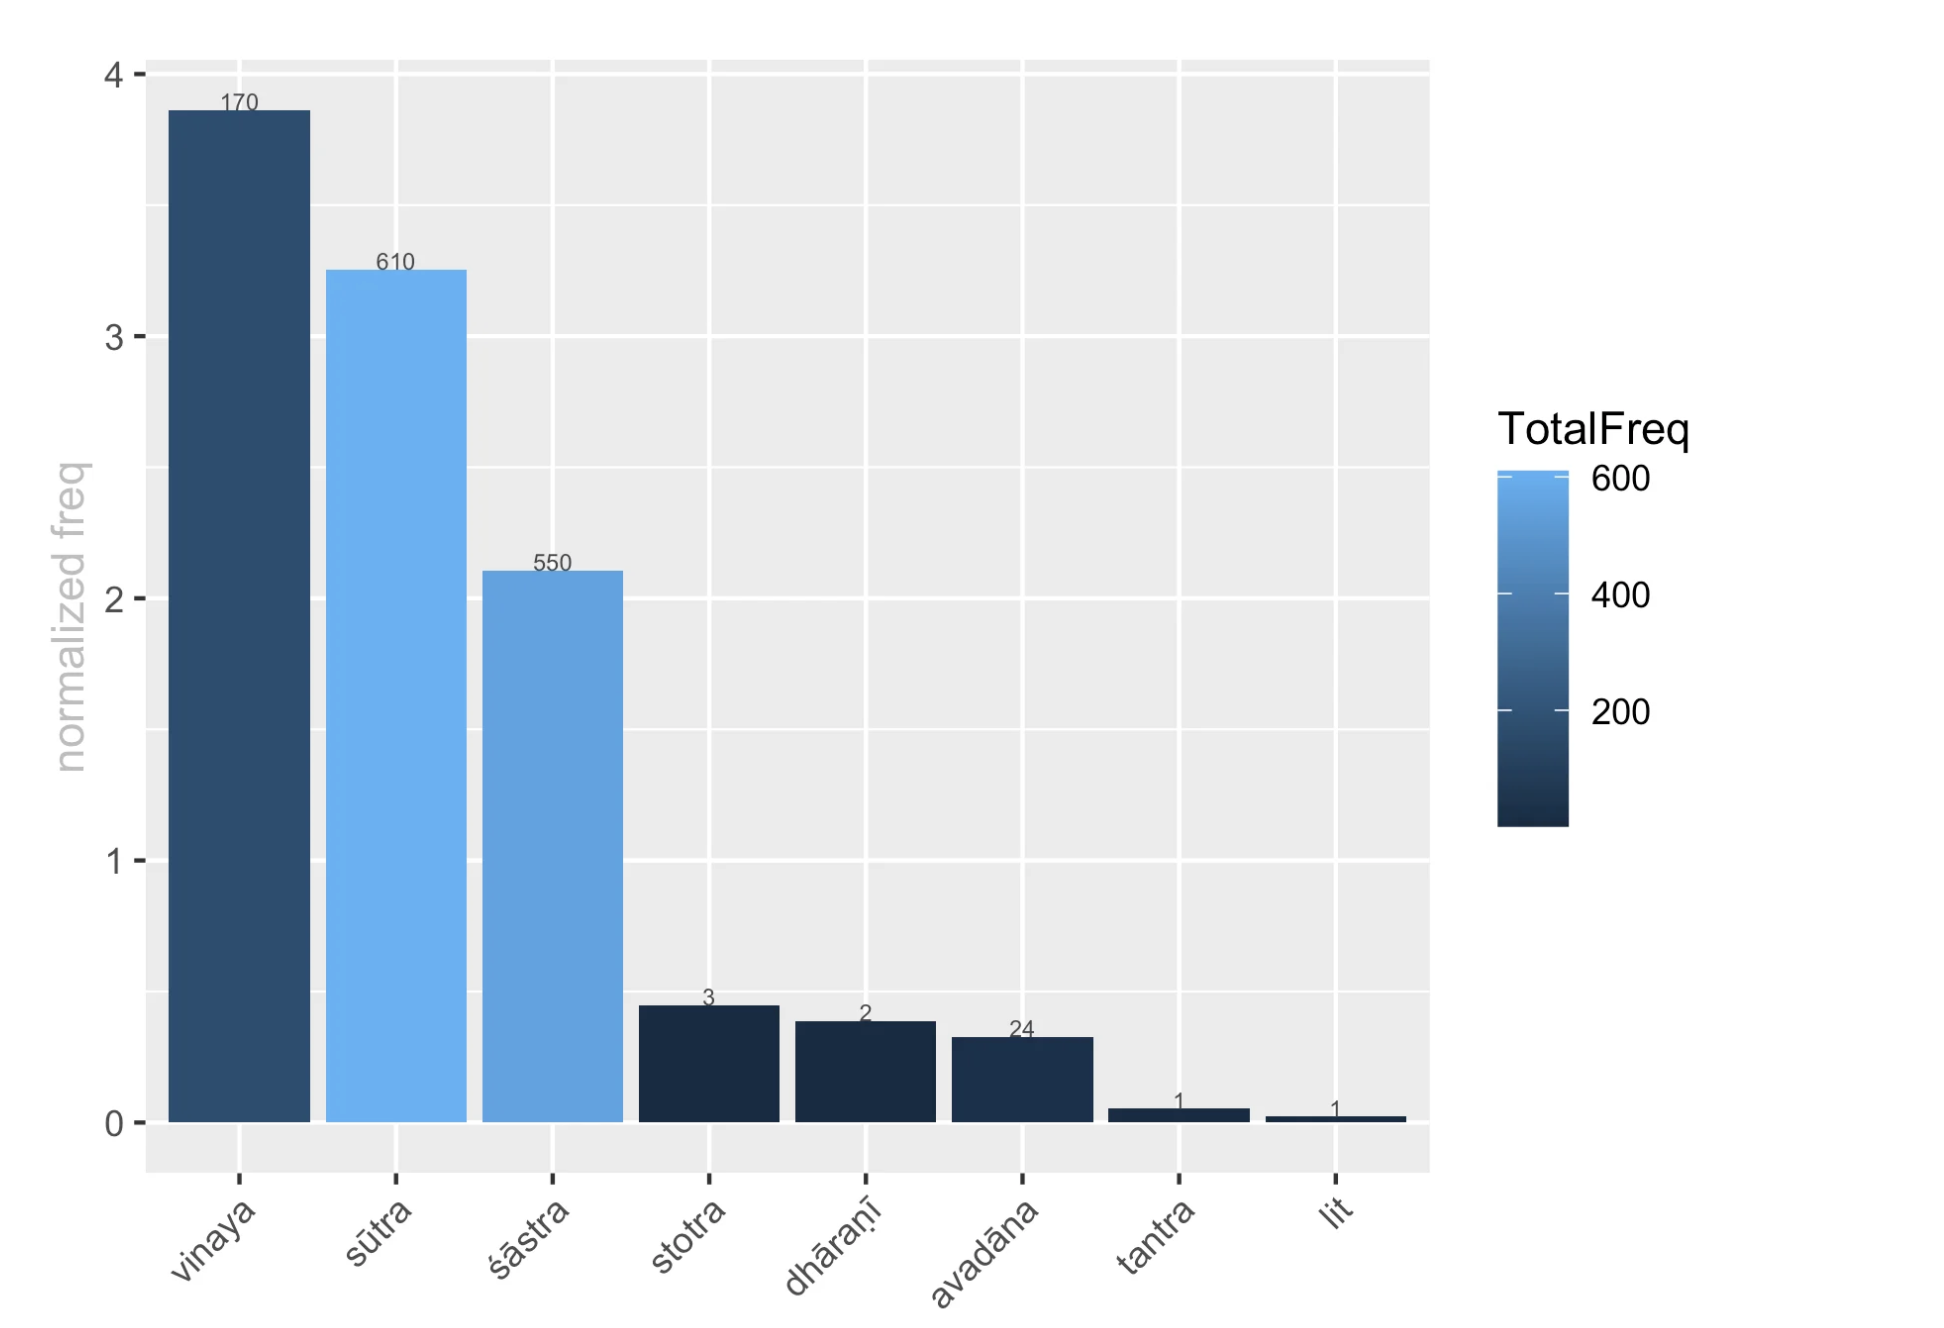
\includegraphics{./www/FreqByGenre_prajJapti.png}

}

\caption{\label{fig-freqbygenre}frequencies normalized by 10k words}

\end{figure}

\hypertarget{sec-freqbytext}{%
\subsubsection{by text}\label{sec-freqbytext}}

\marginnote{\begin{footnotesize}

The texts are arranged in decreasing order of absolute frequency, left
to right. The height of the bars in the charts indicates the normalized
frequency of the lemma per 10,000 words, the colour of the bars
indicates the absolute frequency. The brighter the colour, the highest
the absolute frequency of the lemma. Hover on bars to see title and
frequency information.

\end{footnotesize}}

\hypertarget{info}{%
\subsubsection{info}\label{info}}

Frequency is calculated over the \textasciitilde7-million words
Segmented Corpus of Buddhist Sanskrit (10.5281/zenodo.3457822), as
opposed to the smaller corpus used for semantic annotations in the
Visual Dictionary and Thesaurus of Buddhist Sanskrit (see dictionary
documentation for details).

The height of the bars in the charts indicates the normalized frequency
of the lemma per 10,000 words, the colour of the bars indicates the
absolute frequency (i.e.~the relative size of the texts/corpus in which
the word occurs is not taken into account). The brighter the colour, the
highest the absolute frequency of the lemma. The absolute frequency of
the lemma is also reported in the numbers on top of each bar.

\hypertarget{sec-context}{%
\section{context}\label{sec-context}}

Prajñapti's polysemy is reflected in the variety of contexts in which it
occurs.

The sense of designating something for a use is typically instantiated
in passages describing the preparations made for hosting an assembly and
accompanied by the collocate āsana, although a wider range of words can
be governed by prajñapti in this sense (see also the cognate prajñapta,
which expresses a similar sense).

In the specialized sense of nominal existence, prajñapti occurs in the
context of ontological discussions, where it is usually contrasted with
dravya and accompanied by sat, as well as words associated with key
Buddhist ontological issues, such as pudgala and skandha.

A similar, but broader context frames prajñapti's instantiations of the
senses verbal expression/notion and designation, both of which typically
occur in passages related to the Mahāyāna discourse on language. Here,
prajñapti tends to be accompanied by the usual lexical markers of
Mahāyāna reflections on reality, such as dharmatā and mātra, as well as
by its near-synonyms saṃjñā, vyavahāra and saṃketa. In this regard, it
is important to note that while prajñapti is semantically and
contextually close to both vyavahāra and saṃketa, the idea of
conventionality is less central to prajñapti than to these two words.
Contrary to vyavahāra and saṃketa, prajñapti foregrounds the purely
communicative aspect of verbalization, rather than its social and
transactional dimensions.

\marginnote{\begin{footnotesize}

Bodhicaryāvatāra (2.63: prakṛtyā yac ca sāvadyaṃ prajñapty\^{}āvadyam
eva ca): `péché contre la loi naturelle, péché contre les lois de la
Confrérie'.

The meaning of `precepts', or more generally exposition/formulation, is
the most widely spread of prajñapti's senses in our corpus, and it is
especially prominent in the context of vinaya literature

\end{footnotesize}}

Verses that contrast prajñapti with prakṛti have sometimes been taken as
evidence for interpreting this lemma as denoting what is conventional as
opposed to what is natural (notably Edgerton sub voce prajñapti).
However, one set of these verses, Śikṣāsamuccaya 192.13 (na teṣām
a-sāmarthye api prakṛti-duṣṭatvād gṛhāvāsasya ca prajñapti-sāvadyatvād
iti //), depicts the houselder's life as `blameworthy' by prajñapti, and
it is doubtful that such way of life was considered `blameworthy by
convention' (Edgerton's rendition) in ancient India. `Precepts' may be a
more natural interpretion of prajñapti here, in line with de la Vallee
Poussin's translation of a similar stanza in the Bodhicaryāvatāra (2.63:
prakṛtyā yac ca sāvadyaṃ prajñapty\^{}āvadyam eva ca): `péché contre la
loi naturelle, péché contre les lois de la Confrérie'.

The meaning of `precepts', or more generally exposition/formulation, is
the most widely spread of prajñapti's senses in our corpus, and it is
especially prominent in the context of vinaya literature. Here,
pācattika is a notable collocate. In other genres, the words
contextually associated with prajñapti in this sense are mostly verbs
meaning teaching, such as upadiś. ''

\hypertarget{keywords}{%
\subsubsection{keywords}\label{keywords}}

\marginnote{\begin{footnotesize}

The size of words in the wordcloud is proportional to the Log Ratio.
(for information on this statistics see Hardie 2014 )

words in red occur together with the lemma in at least 10\% of the
texts. the number that shows when hovering over the words is the Log
Ratio.

\end{footnotesize}}

\hypertarget{info-1}{%
\subsubsection{info}\label{info-1}}

the wordcloud displays words that are statitistically over-represented
in the immediate context of the lemma (defined as the words that occur
in the same sentence as the lemma), compared to their overall frequency
in the rest of the \textasciitilde7-million words Segmented Corpus of
Buddhist Sanskrit.

The statistics used for keyness are Log Likelyhood over 10, Log Ratio
over 2. For the sake of readability, only keywords that occur at least
20 times in the lemma's citations are included in the wordcloud and
table.

The size of words in the wordcloud is proportional to the Log Ratio.
(for information on this statistics see Hardie 2014 )

words in red occur together with the lemma in at least 10\% of the
texts. the number that shows when hovering over the words is the Log
Ratio.

\hypertarget{sec-connotation}{%
\section{connotation}\label{sec-connotation}}

Overall, prajñapti has a neutral connotation.

However, when it expresses the meaning of exposition/formulation,
especially in the context of the Buddha's teaching, it is sometimes
surrounded by words with a markedly positive connation. These words lend
a positive semantic prosody to prajñapti in about 20\% of the citations
that we manually annotated with this sense (in yellow in the chart).

By contrast, when it expresses the meanings of verbal expression/notion
and nominal existence, prajñapti acquires a slighly negative semantic
prosody in about 30\% of the citations we annotated (in pale red in the
graph). The negative tinge mostly derives from emphasis on the `mere'
nominal value and illusoriness of entities that exist by way of
prajñapti.

\marginnote{\begin{footnotesize}

semantic prosody (sem.pros) here refers to whether a lemma acquires a
positive or negative overtone in context.

\end{footnotesize}}

\hypertarget{semantic-prosody-proportion}{%
\subsubsection{semantic prosody
proportion}\label{semantic-prosody-proportion}}

\marginnote{\begin{footnotesize}

The barcharts are based on manually annotated data. Please refer to the
documentation of A Visual Dictionary and Thesaurus of Buddhist Sanskrit
for information on the corpus and sampling frame used.

\end{footnotesize}}

\hypertarget{absolute-freq}{%
\subsubsection{absolute freq}\label{absolute-freq}}

\hypertarget{info-2}{%
\subsubsection{info}\label{info-2}}

The barcharts are based on manually annotated data.

Please refer to the documentation of A Visual Dictionary and Thesaurus
of Buddhist Sanskrit for information on the corpus and sampling frame
used.

semantic prosody (sem.pros) here refers to whether a lemma acquires a
positive or negative overtone in context. Generally the semantic prosody
associated to a word emerges from a repeated pattern of use. For example
we can say that `set in' has a negative connotation in English because
it is systematically associated with words that possess a negative
connotation (Louw 1993). For a pattern to emerge, we need to consider
many individual instances. To this end in this project we treat semantic
prosody slightly differently and we annotate it in each citation as a
property of each instantiation of a lemma in context.

We use a fourfold typology for semantic prosody: positive, negative,
neutral and neutral-nagative. We annotate a lemma as having negative
semantic prosody when the concept expressed by the lemma is clearly
depicted as negative , e.g.~the lemma vikalpa in the phrase
vikalpasaṃsārāvahāka (vikalpa is the source of saṃsāra).

Conversely, we annotate semantic prosody as positive if the concept
expressed by a lemma is described as positive, or leading to something
good etc. In cases where the lemma is negated (e.g.~na vikalpayati) or
is modified by an adjective with a negative connotation which suggests
that some aspects of the concept expressed by the lemma are negative (
but not the concept tout-court, e.g.~akuśala-vikalpa), we annotate the
semantic prosody as being neutral-negative.

Given the rarity of positive semantic prosody in the vocabulary explored
in the Visual Dictionary and Thesaurus of Buddhist Sanskrit we
categorize all positive occurrences as pos, even when they would better
lend themselves to neu.pos, for analogy with neu.neg above.

\hypertarget{semantic-prosody-examples}{%
\subsection{semantic prosody examples}\label{semantic-prosody-examples}}

\hypertarget{sec-examplesemprospos}{%
\subsubsection{positive}\label{sec-examplesemprospos}}

\textbf{pratibhāna-pratisaṃvidā
yathā-\emph{prajñapty}-a-vikopanatay\^{}ā-paryantatayā dharmaṃ deśayati
//} {[}daśabhūmikasūtra, 51{]}\\
``By the analytical knowledge of eloquence he teaches doctrine with
unshaken infinitude as his ideation.'' {[}Honda 245-6{]}

\hypertarget{sec-examplesemprosneg}{%
\subsubsection{negative}\label{sec-examplesemprosneg}}

\textbf{yath\^{}oktam ātmā ātm\^{}eti bhikṣavo bālo 'śrutavān
pṛthagjanaḥ \emph{prajñaptim} anupatito na tv atr\^{}ātmā vā ātmīyaṃ vā
iti /}{[}abhidharmakośabhāṣya, 140{]}\\
``It is said in fact, `The fool, the ignorant, the Pṛthagjana,
conforming to the manners of vulgar speech, thinks ``me,'' or ``mine;''
but there is not any ``me'' or ``mine.''\,'\,'' {[}Pruden 419{]}

\hypertarget{sec-examplesemprosneu}{%
\subsubsection{neu}\label{sec-examplesemprosneu}}

\textbf{kiṃ kāraṇaṃ pratyutpanne adhvani
śrāvaka-pratyekabuddha-bodhisattvānāṃ \emph{prajñaptiḥ} prajñapyate ?}
{[}saddharmapuṇḍarīka, 91{]}\\
``\ldots for what reason then is the designation of disciples
(Srāvakas), Buddhas, and Bodhisattvas kept up in the present times?''
{[}Kern 129{]}

\hypertarget{sec-examplesemprosneuneg}{%
\subsubsection{neu.neg}\label{sec-examplesemprosneuneg}}

\textbf{sarva-\emph{prajñapti}-samatikrāntaṃ lokottaram ity ucyate
/}{[}suvikrāntavikrāmiparipṛcchā, 4{]}\\
``\ldots one speaks of the `supramundane' as of that which has
completely transcended all verbal concepts.''{[}Conze 5{]}
``prajñapti68suvikrāntavikrāmiparipṛcchā''

\hypertarget{examples}{%
\section{examples}\label{examples}}

\hypertarget{sec-examplesnominalexistence}{%
\subsection{nominal existence}\label{sec-examplesnominalexistence}}

\textbf{dravya-\emph{prajñapti}-sat-sattva-vikalpau grāhakau matau /
pṛthagjan\^{}-ārya-bhedena pratyekaṃ tau nav\^{}-ātmakau // 5.6 //}
{[}abhisamayālaṃkāra, 5.5{]}\\
``(The Sutra then) considers the two (false) discriminations of the
subject. The one regards beings (or persons) as (real) substantial
entities, the second as (merely) nominal entities. The first refers to
the common people, the second to the saints. Each one consists of nine
items.'' {[}Conze 81{]}

\textbf{kiṃ c\^{}edaṃ dravyata iti kiṃ vā \emph{prajñaptitaḥ} /
rūp\^{}ādivat bhāv\^{}āntaraṃ cet dravyataḥ / kṣīr\^{}ādivat samudāyaś
cet prajñaptitaḥ /} {[}abhidharmakośabhāṣya, 461{]}\\
``Does the pudgala exists as a real entity or as a nominal construct? If
a person is a distinct entity like visible form and other such things,
he is substantially real; but if {[}by analysis{]} he is {[}shown to
be{]} a collection {[}of substances{]}, like milk and other such things,
he is real by way of a conception.'' {[}Duerlinger 73{]}

\hypertarget{sec-examplesdesignation}{%
\subsection{designation}\label{sec-examplesdesignation}}

\textbf{teṣāṃ dāni kumārāṇāṃ śakyaṃ śākiyā ti
samākhyā-samājñā-\emph{prajñapti}udapāsi //} {[}mahāvastu, 1.351{]}\\
``\,`Cunning, sirs, are these princes.' And from the `cunning' of these
princes arose their name, appellation and designation of Śākiyans.''
{[}Jones 297{]}

\textbf{{[}\ldots{]} na ca saṃsthānaṃ paramāṇau vidyate dīrgh\^{}ādi /
tasmād bahuṣv eva tathā saṃniviṣṭeṣu dīrgh\^{}ādi-\emph{prajñaptiḥ} /
atha mataṃ saṃsthāna-paramāṇava eva tathā saṃniviṣṭā
dīrgh\^{}ādi-saṃjñāṃ labhanta iti /}{[}abhidharmakośabhāṣya, 195{]}\\
``There is no atom of length. {[}\ldots{]} Therefore what we designate
as long is a number of real things,---atoms of color,---arranged in a
certain manner.'' {[}Pruden 557-8{]}

\textbf{idaṃ ca nāma saṃjñā prajñaptiś cakṣur iti / etac ca vastu-mātram
/ yatr\^{}edaṃ nāma saṃjñā \emph{prajñaptiḥ} / n\^{}āta uttari n\^{}āto
bhūyaḥ /}{[}bodhisattvabhūmi, 273{]}\\
``{[}One is,{]} `This is the name, the appellation, and the designation
``eye,''\,' and {[}the other is,{]} `That is the bare substance in
relation to which this name, appellation, and designation {[}occur{]}.'
There is nothing beyond that and nothing more than that.'' {[}Engle
643{]}

\textbf{yadā ca te kulaputra tasmin sva-nāmni āgantuka-saṃjñā utpannā
bhavati pratilabdhā sa tvaṃ yā te cakṣuṣi cakṣur-nāma cakṣuḥ-saṃjñā
cakṣuḥ-\emph{prajñaptis} tām apy adhyātmaṃ yoniśo manasi-kuru /}
{[}bodhisattvabhūmi, 273{]}\\
``O child of good family, when this conception of being adventitious has
arisen in you and been understood {[}by you{]} in relation to your name,
then also direct your attention inwardly in a proper manner to the name
`eye,' the appellation `eye,' and the designation `eye' {[}that occur{]}
in relation to your eye.'' {[}Engle 643{]}

\hypertarget{sec-examplesverbalexpression}{%
\subsection{verbal expression
notion}\label{sec-examplesverbalexpression}}

\textbf{{[}\ldots{]} na ca saṃsthānaṃ paramāṇau vidyate dīrgh\^{}ādi /
tasmād bahuṣv eva tathā saṃniviṣṭeṣu dīrgh\^{}ādi-\emph{prajñaptiḥ} /
atha mataṃ saṃsthāna-paramāṇava eva tathā saṃniviṣṭā
dīrgh\^{}ādi-saṃjñāṃ labhanta iti /}{[}abhidharmakośabhāṣya, 195{]}\\
``There is no atom of length. {[}\ldots{]} Therefore what we designate
as long is a number of real things, atoms of color, arranged in a
certain manner.'' {[}Pruden 557-8{]}

\textbf{yadā na bhavati saṃjñā samajñā \emph{prajñaptir} vyavahāraḥ /
tadā prajñāpāramit\^{}ety ucyate //} {[}aṣṭasāhasrikā, 89{]}\\
``Where there is no perception, appellation, conception or conventional
expression, there one speaks of `perfection of wisdom.'\,'' {[}Conze
138{]}

\textbf{jīvit\^{}endriyaṃ katamat / nikāya-sabhāge
pūrva-karm\^{}-āviddhe sthiti-kāla-niyame āyur iti \emph{prajñaptiḥ} //}
{[}abhidharmasamuccaya, 18{]}\\
``What is the life faculty? Life span designates a period of fixed
duration affected by former actions in the similarity of types?''
{[}Boin-Webb 19{]}

\textbf{sarva-\emph{prajñapti}-samatikrāntaṃ lokottaram ity ucyate
/}{[}suvikrāntavikrāmiparipṛcchā, 4{]}\\
``\ldots one speaks of the `supramundane' as of that which has
completely transcended all verbal concepts.''{[}Conze 5{]}

\textbf{yath\^{}oktam ātmā ātm\^{}eti bhikṣavo bālo 'śrutavān
pṛthagjanaḥ \emph{prajñaptim} anupatito na tv atr\^{}ātmā vā ātmīyaṃ vā
iti /} {[}abhidharmakośabhāṣya, 140{]}\\
``It is said in fact, `The fool, the ignorant, the Pṛthagjana,
conforming to the manners of vulgar speech, thinks ``me,'' or ``mine;''
but there is not any ``me'' or ``mine.''\,'\,'' {[}Pruden 419{]}

\hypertarget{appointing}{%
\subsection{appointing}\label{appointing}}

**bahir nagarasya pañca vihāra-śatāni kāritāni pañca
mañca-pīṭha-vṛṣi-koccaka-bimbopadhāna-caturasraka-śatāni dāpitāni pañca
piṇḍapāta-śatāni prajñaptāni vistīrṇ\^{}-āvakāśe ca pṛthivī-pradeśe
āsana-\emph{prajñaptiḥ} *kāritā /**{[}divyāvadāna\_selection,
468.017{]}\\
``He also commissioned five hundred monastic dwellings outside of the
city; gave out five hundred chairs, seats, cushions, woolen blankets,
pillows, and shawls; distributed five hundred meals; and had a seat
specially prepared for the venerable Mahākātyāyana in a wide-open tract
of land.'' {[}Rotman{]}

\hypertarget{title-of-treatise}{%
\subsection{title of Treatise}\label{title-of-treatise}}

\textbf{\emph{prajñaptau}} \textbf{tu pratisaṃvidām eva nirdeśaḥ /}
{[}abhidharmakośabhāṣya, 419{]}\\
``According to the Prajñaptipāda, the Unhindered Knowledges are in the
following order: {[}\ldots{]}.'' {[}Pruden 1154{]}

\hypertarget{formulationexposition}{%
\subsection{formulation/exposition}\label{formulationexposition}}

\textbf{kathaṃ tāvad eṣām upāsaka-saṃvar\^{}ādīnām aṅga-pratiniyamo
bhavati / śāstṛ-\emph{prajñapti}-vaśāt /} {[}abhidharmakośabhāṣya,
216{]}\\
``Answer: How can we know the extent, the number of the rules of the
disciplines of the Upasaka, the Sramanera, or the Bhiksu? Evidently
through the teaching of the Master.'' {[}Pruden 600{]}

\textbf{a-karkaśā śikṣā-\emph{prajñapt}i-sukh\^{}opāyatvāt /}
{[}mahāyānasūtrālaṃkāra, 80{]}\\
``It is `without harshness' because it has the art of pleasantly
announcing the precepts.'' {[}Thurman 157{]}

\textbf{\ldots{} iti svayan na upasampādayet niḥsargika-pācattikaṃ /
yāvat \emph{prajñaptiḥ}/} {[}bhikṣuṇīvinaya, 179{]}\\
``C'est une faute entraînant abandon {[}de l'objet en cause{]} et aveu
formel -etc \ldots{} promulgation.'' {[}Nolot 178{]}

\textbf{mayā bālena mūḍhena yat kiṃcit pāpam ācitaṃ / prakṛtyā yac ca
sāvadyaṃ \emph{prajñapty}\^{}āvadyam eva ca //} {[}bodhicaryāvatāra,
2.63{]}\\
``Le péché que ma sottise et mon égarement ont accumulé, péché contre la
loi naturelle, péché contre les lois de la Confrérie, {[}\ldots{]}.''
{[}La Vallée Poussin 452,31-33{]}

\bookmarksetup{startatroot}

\hypertarget{vitarka}{%
\chapter{vitarka}\label{vitarka}}

{\marginnote{\begin{footnotesize}\emph{khinnasya suptasya ca nirvṛtasya
bādhaṃ yathā saṃjanayanti śabdāḥ / adhyātmam aikāgryam upāgatasya
bhavanti bādhāya tathā} vitarkāḥ // {[}saundarananda, 17.46{]} ``As
noises harass a man who is tired and soundly asleep, so thoughts harass
the man who has attained internal concentration.'' {[}Johnston
106{]}\end{footnotesize}}}

Vitarka belongs to the semantic domain of Thought. More specifically,
vitarka is thought that surfaces to our attention spontaneously (thought
esp.~spontaneous \& distracting), typically triggered by sense
impressions, memories, or desires.

Many occurrences imply a tinge of lust or malice. For example, vitarka
often indicates thoughts that linger on the prospect of meeting an
attractive partner or, more darkly, on the prospect of violence. Whether
these thoughts amount to fantasising, scheming, or engaging in a mental
dialogue over the matter at hand is not clear. It is likely that vitarka
was rather vague regarding this point, lending itself to take on all
these different semantic nuances depending on context. The one aspect of
thought that vitarka appears to foreground in non-specialised contexts
is its unwitting, unintentional nature, with vitarka being typically
characterized as distracting.

The unfocussed nature of vitarka is at the root of its terminological
uses as the first dhyānāṅga and as a caitasika dharma. In the former
application, vitarka denotes the initial, unfoccused, phase in mental
progression that leads to meditative absorption . In the latter, it
denotes a neutral mental factor traditionally held responsible for the
initial steering of the mind towards an object of thought . These two
meanings often overlap, since the caitasika dharma can function as the
first dhyānāṅga. Hence we have merged these two specialized applications
under the single label `a caitasika dharma'

\begin{figure}

{\centering 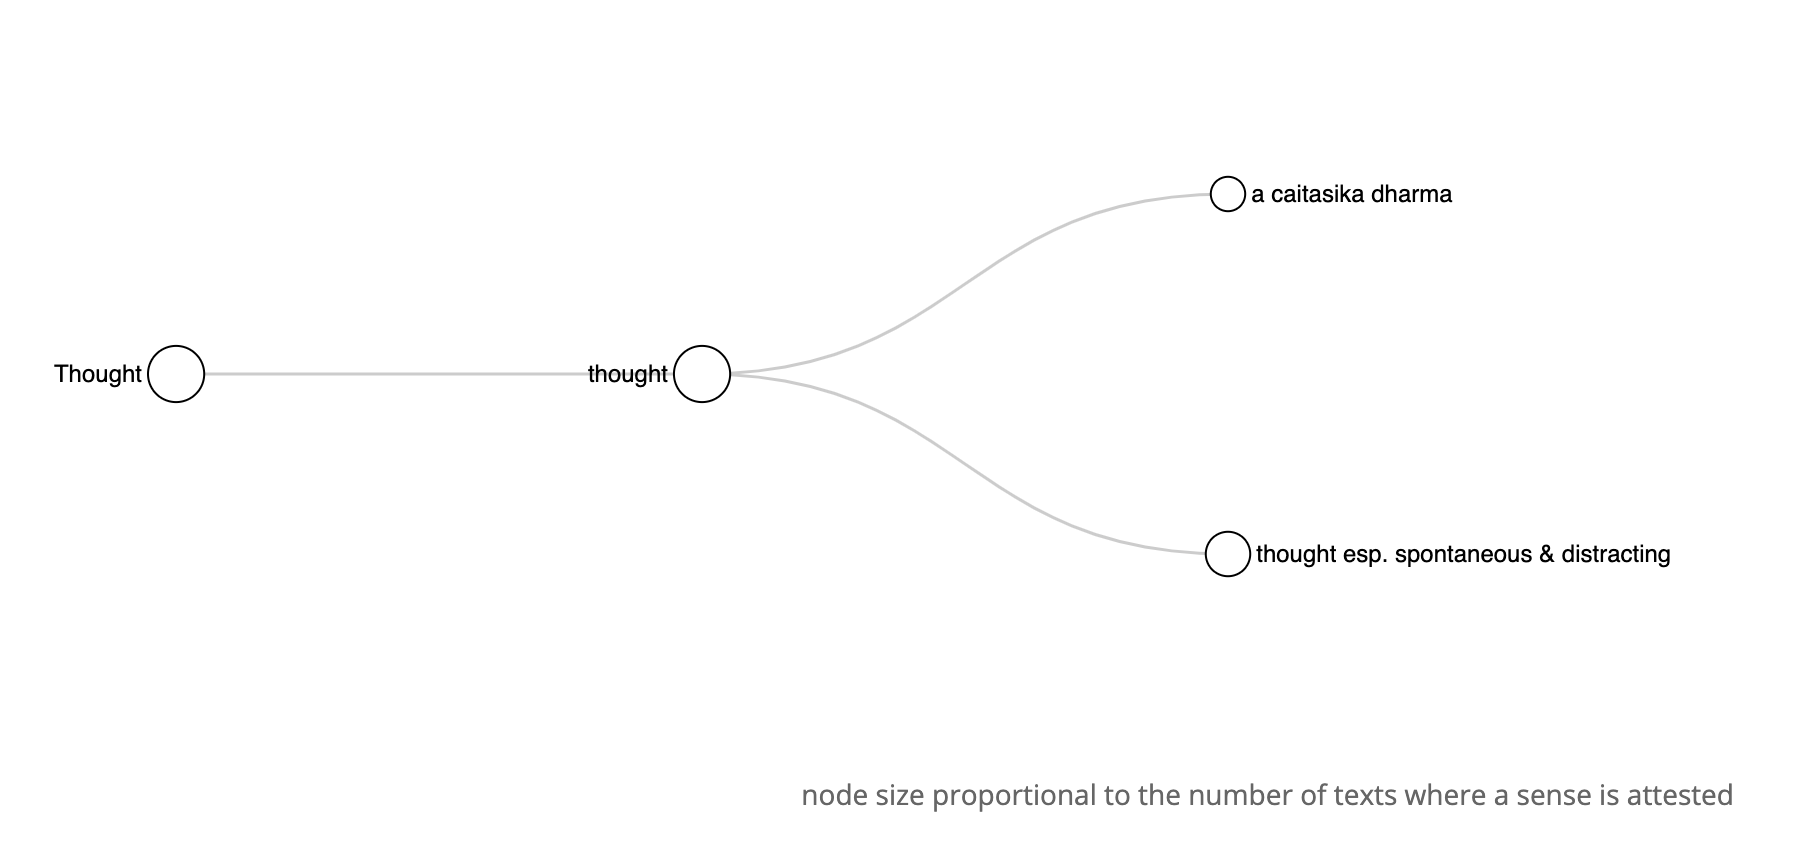
\includegraphics{./www/semanticTree_vitarka.png}

}

\caption{\label{fig-semantictree}semantic tree}

\end{figure}

\hypertarget{frequency}{%
\section{frequency}\label{frequency}}

Vitarka is a mid-frequency word in our corpus; both relative to all
words in the corpus and relative specifically to words expressing the
concept of thinking (note the position of vitarka on the word-frequency
curve in the frequency graph ).

It is fairly uniformly distributed over all the diachronic layers
considered in this dictionary. Indeed vitarka is more evenly distributed
across both periods and genres than most words in our corpus (see
dispersion graphs on the right, or in the dispersion tabs below; the
fact that vitarka falls below the horizontal like indicates it is more
evenly dispersed than the average word in our corpus).

\begin{marginfigure}

{\centering \includegraphics{./www/genreDP_vitarka.webp}

}

\caption{genre dispersion}

\end{marginfigure}

Yet, despite being attested in all kinds of literature, its distribution
over different genres is far from homogeneous, with its use definitely
most prominent in śāstras (see sense by genre tab).''

\hypertarget{sec-freqcurve}{%
\subsubsection{freq graph}\label{sec-freqcurve}}

\marginnote{\begin{footnotesize}

Frequency and dispersion are calculated over the
\textasciitilde7-million words Segmented Corpus of Buddhist Sanskrit
(10.5281/zenodo.3457822).

Dispersion is calculated with Gries' deviation of proportion formula
(Gries, S. 2008. Dispersion and adjusted frquencies in corpora.
International Journal of Corpus Linguistics, 13(4): 403-437)

\end{footnotesize}}

\begin{figure}

{\centering \includegraphics{./www/ZipfCurveFreq_vitarka.webp}

}

\caption{\label{fig-freqcurve}lemma's frequency compared to
near-synonyms}

\end{figure}

\hypertarget{sec-genredp1}{%
\subsubsection{genre dispersion}\label{sec-genredp1}}

\marginnote{\begin{footnotesize}

Frequency and dispersion are calculated over the
\textasciitilde7-million words Segmented Corpus of Buddhist Sanskrit
(10.5281/zenodo.3457822).

Dispersion is calculated with Gries' deviation of proportion formula
(Gries, S. 2008. Dispersion and adjusted frquencies in corpora.
International Journal of Corpus Linguistics, 13(4): 403-437)

\end{footnotesize}}

\begin{figure}

{\centering \includegraphics{./www/genreDP_vitarka.webp}

}

\caption{\label{fig-genredp1}genre dispersion}

\end{figure}

\hypertarget{sec-perioddp1}{%
\subsubsection{period disp.}\label{sec-perioddp1}}

\marginnote{\begin{footnotesize}

Frequency and dispersion are calculated over the
\textasciitilde7-million words Segmented Corpus of Buddhist Sanskrit
(10.5281/zenodo.3457822).

Dispersion is calculated with Gries' deviation of proportion formula
(Gries, S. 2008. Dispersion and adjusted frequencies in corpora.
International Journal of Corpus Linguistics, 13(4): 403-437)

\end{footnotesize}}

\begin{figure}

{\centering \includegraphics{./www/periodDP_vitarka.webp}

}

\caption{\label{fig-perioddp1}period dispersion}

\end{figure}

\hypertarget{sec-sensebygenre}{%
\subsubsection{sense by genre}\label{sec-sensebygenre}}

\begin{figure*}

{\centering 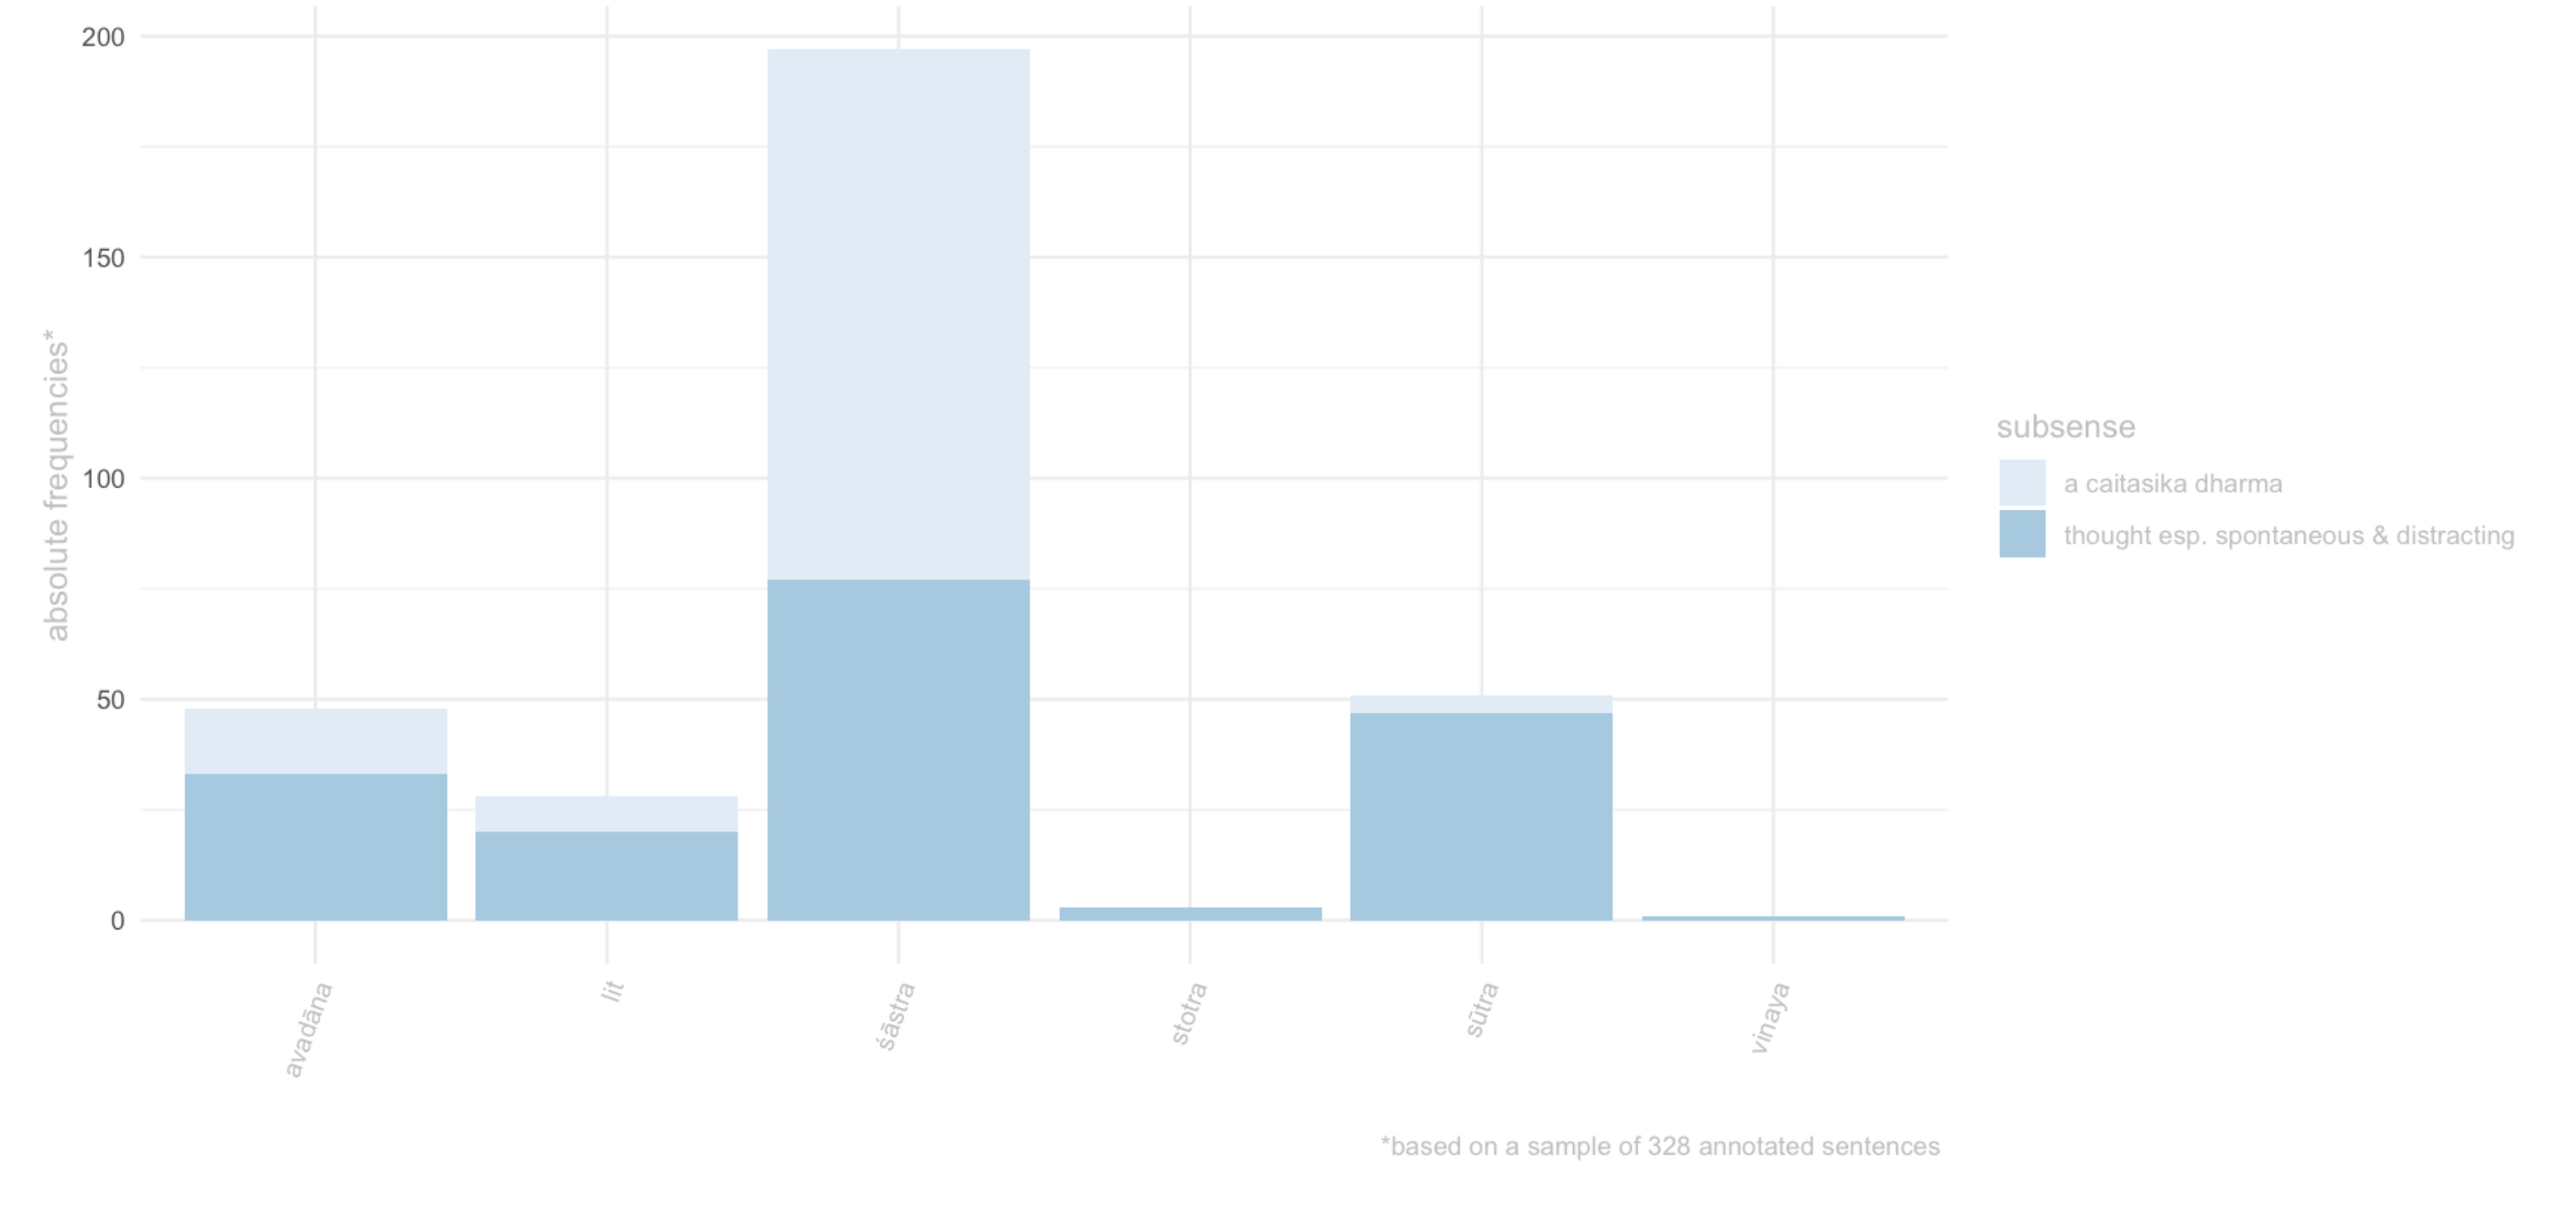
\includegraphics{./www/SenseByGenre_vitarka.png}

}

\caption{\label{fig-sensebygenre}sense by genre}

\end{figure*}

\hypertarget{sec-disperioninfo}{%
\subsubsection{info}\label{sec-disperioninfo}}

frequency and dispersion are calculated over the
\textasciitilde7-million words Segmented Corpus of Buddhist Sanskrit
(10.5281/zenodo.3457822), as opposed to the smaller corpus used for the
Visual Dictionary and Thesaurus of Buddhist Sanskrit (see dictionary
documentation for details).

For the sake of readability, only words occurring at least 5 times in
the corpus have been plotted on the frequency and dispersion curves.

Dispersion is calculated with Gries' deviation of proportion formula
(Gries, S. 2008. Dispersion and adjusted frquencies in corpora.
International Journal of Corpus Linguistics, 13(4): 403-437).

the sense by genre plot is based on a sample of sentences that we have
manually annotated with semantic information for the Visual Dictionary
and Thesaurus of Buddhist Sanskrit. For details about our sampling and
annotation procedures see the dictionary documentation page.

\hypertarget{sec-register}{%
\section{register}\label{sec-register}}

Vitarka occurs much more frequently in śāstra than in any other genre
(526 occurrences per million words in śāstra and about 100 or less for
the other genres). About two thirds of all attestations of this word in
the Segmented Buddhist Sanskrit Corpus occur in śāstras (422 out of 637
attestations). This does not necessarily indicate that vitarka
gravitates towards the philosophical or technical register. Attestations
of the word vitarka in narrative and non-specialized contexts suggest
that the use of this word is not restricted to the philosophical
discourse, with the every-day character of some attestations even
tilting towards a general language feel, e.g.~:

\begin{quote}
If a man, moved by considerations of greed, had made a date with a
handsome, attractive and good-looking woman, and if now that woman were
held back by someone else and could not leave her house, what do you
think, Subhuti, with what would that man's preoccupations be connected?
Subhuti: With the woman, of course. He thinks about her coming, about
the things they will do together, and about the joy, fun and delight he
will have with her. The Lord: Will he have many such ideas in the course
of a day? Subhuti: Many indeed, O Lord. {[}Conze, 210{]} (tadyathāpi
nāma subhūte kaścid eva puruṣo rāgacarito vitarkacaritaḥ \textbar{}
tasya puruṣasya rāgacaritasya vitarkacaritasya striyā abhirūpayā
prāsādikayā darśanīyayā saha saṃketaḥ kṛto bhavet \textbar{} sā khalu
punaḥ strī paraparigṛhītā bhavet \textbar{} na vaśayed ātmānamagārān
niṣkramitum \textbar{} tat kiṃ manyase subhūte kiṃ pratisaṃyuktās tasya
puruṣasya vitarkāḥ pravarteran? subhūtir āha - strīpratisaṃyuktā eva
bhagavaṃs tasya puruṣasya vitarkāḥ pravarteran - iyam āgacchati, iyam
āgatā \textbar{} tayā sārdham evaṃ kariṣyāmi, evaṃ ramiṣyāmi, evaṃ
krīḍiṣyāmi, evaṃ pravicārayiṣyāmīti \textbar{} bhagavān āha - tat kiṃ
manyase subhūte divasasyātyayena tasya puruṣasya kiyanto
vitarkotpadyeran? subhūtir āha - bahavo bhagavan divasasyātyayena tasya
puruṣasya vitarkotpadyeran \ldots{} {[}Aṣṭasāhasrikāprajñāpāramitā:
Vaidya, 170-171{]}).
\end{quote}

\hypertarget{fequency-by-genre}{%
\subsubsection{fequency by genre}\label{fequency-by-genre}}

\marginnote{\begin{footnotesize}

The height of the bars in the charts indicates the normalized frequency
of the lemma per 10,000 words, the colour of the bars indicates the
absolute frequency.

\end{footnotesize}}

\begin{figure}

{\centering 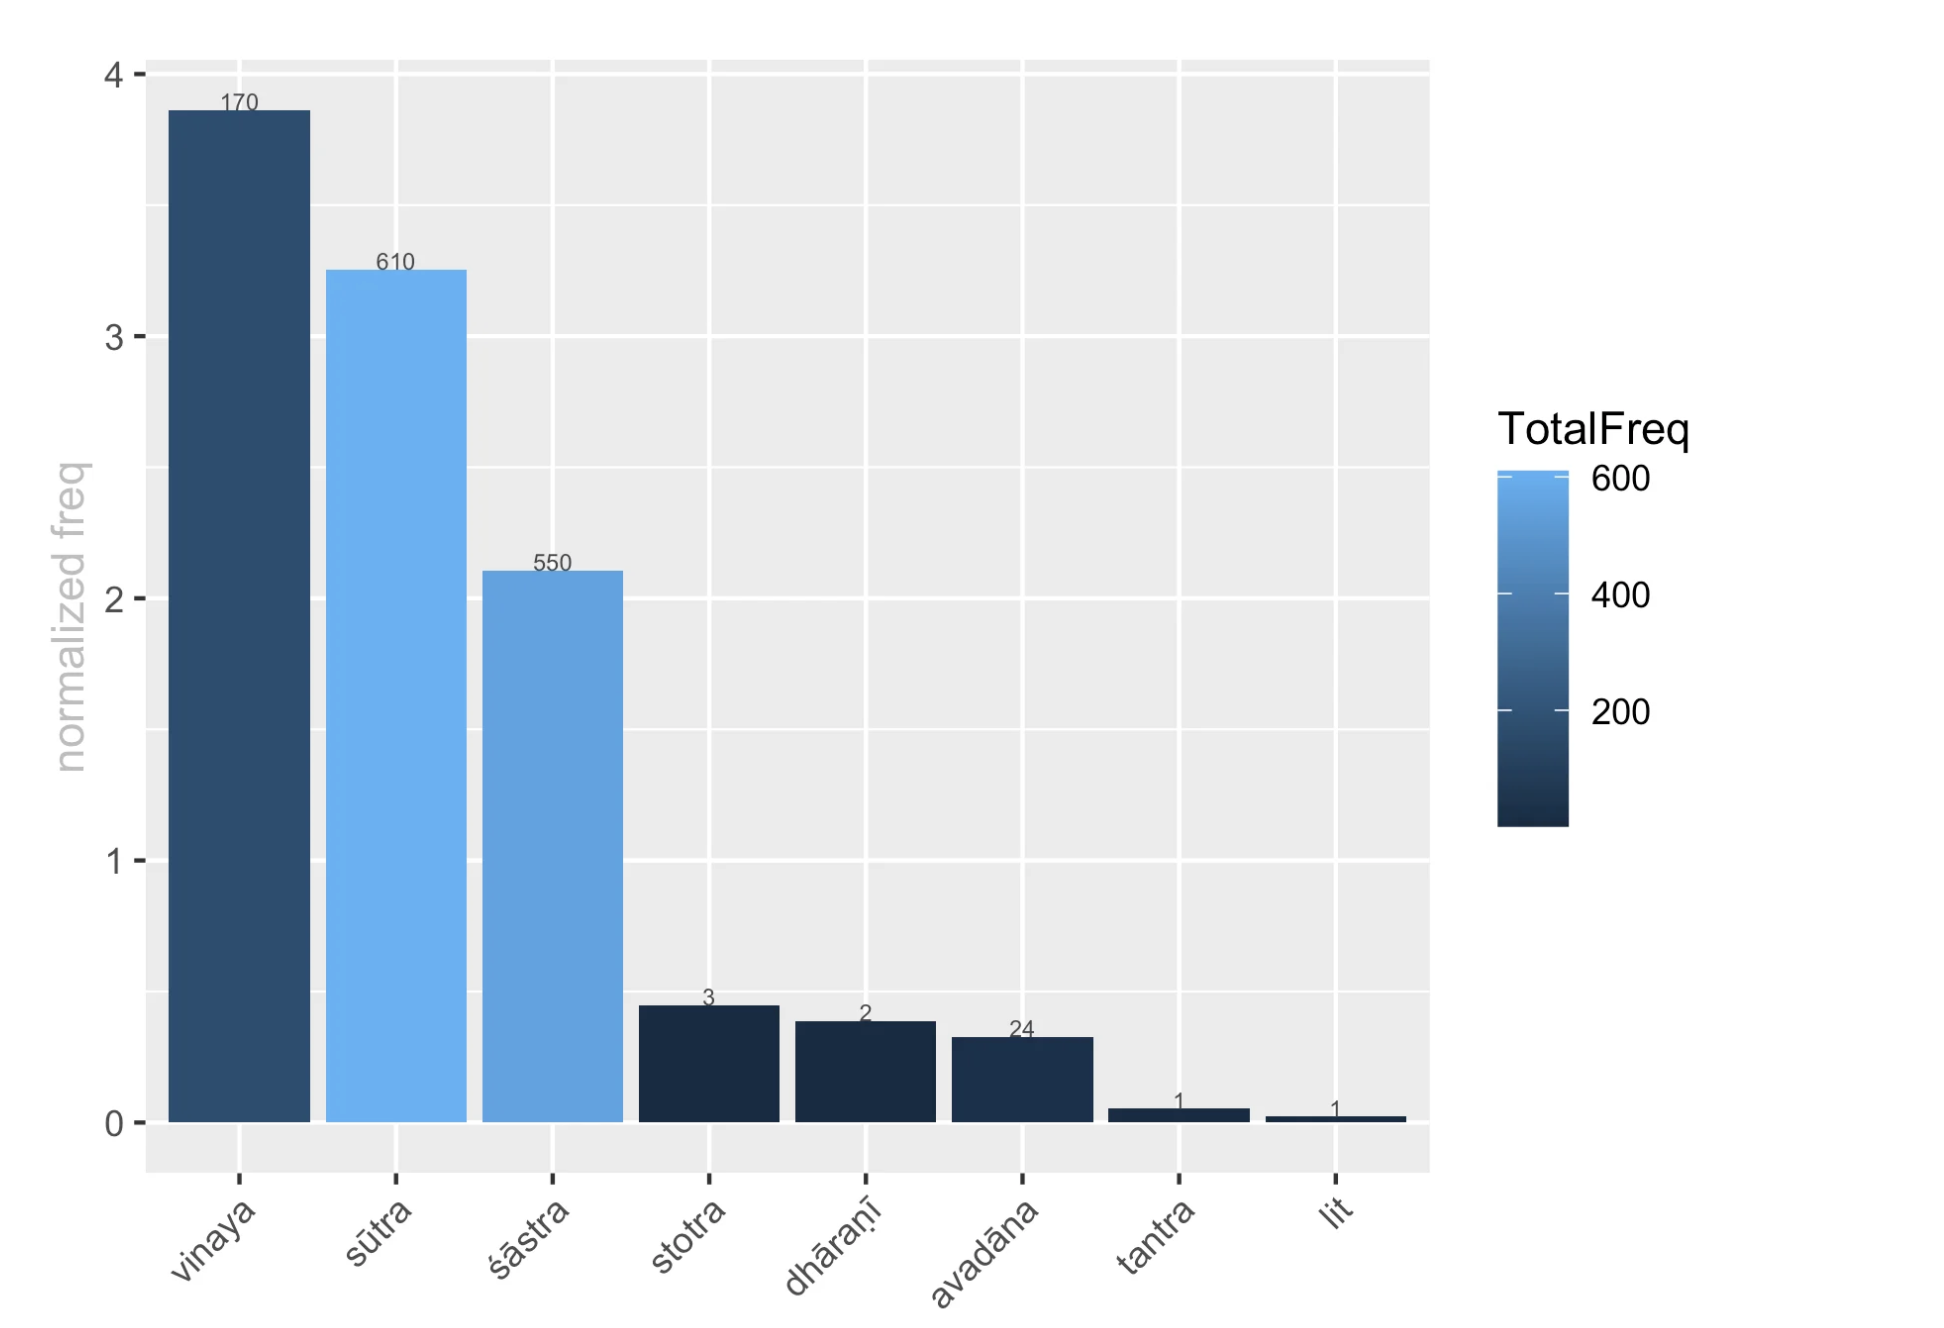
\includegraphics{./www/FreqByGenre_prajJapti.png}

}

\caption{\label{fig-freqbygenre}frequencies normalized by 10k words}

\end{figure}

\hypertarget{by-text}{%
\subsubsection{by text}\label{by-text}}

\marginnote{\begin{footnotesize}

The texts are arranged in decreasing order of absolute frequency, left
to right. The height of the bars in the charts indicates the normalized
frequency of the lemma per 10,000 words, the colour of the bars
indicates the absolute frequency. The brighter the colour, the highest
the absolute frequency of the lemma. Hover on bars to see title and
frequency information.

\end{footnotesize}}

\hypertarget{info-3}{%
\subsubsection{info}\label{info-3}}

Frequency is calculated over the \textasciitilde7-million words
Segmented Corpus of Buddhist Sanskrit (10.5281/zenodo.3457822), as
opposed to the smaller corpus used for semantic annotations in the
Visual Dictionary and Thesaurus of Buddhist Sanskrit (see dictionary
documentation for details).

The height of the bars in the charts indicates the normalized frequency
of the lemma per 10,000 words, the colour of the bars indicates the
absolute frequency (i.e.~the relative size of the texts/corpus in which
the word occurs is not taken into account). The brighter the colour, the
highest the absolute frequency of the lemma. The absolute frequency of
the lemma is also reported in the numbers on top of each bar.

\hypertarget{sec-context}{%
\section{context}\label{sec-context}}

The predominance in śāstra materials is probably due to two factors.
First, the topic to which this word is associated. That is, the torments
and distractions brought about by worldly attachments, notably love and
desire. As the even diachronic distribution of vitarka suggests, this
topic is close to the core of Buddhist thought and largely unaffected by
the waxing and waning of specific schools and philosophical
controversies.

All kinds of treatises touch upon this matter, especially (but far from
exclusively) in the context of meditation, hence the relatively high
volume of occurrences of this word in sāstras. Some 80\% of the
attestation of vitarka we sampled from the Bodhisattvabhūmi, foreground
this aspect of vitarka.

Second, as mentioned in the introductory paragraph, a `technical' sense
developed from the general senses of vitarka to term one of the
caitasika dharma (and one of the dhyānāṅga). Terminological applications
of the word are responsible for three quarters of the attestations we
sampled from the Abhidharmakośabhāṣya, and is likely to play a major
role in other śastras as well. In its specialized sense, vitarka is
typically accompanied by vicāra, the caitasika dharma that is described
as following vitarka in the chain of mental events leading to meditative
concentration.

The statistically significant collocates of vitarka depicted in the
wordcloud below clearly point to these two uses of vitarka, the more
general sense of distracting lustful thought and the specialized sense
the caitasika dharma precursor of vicāra, and to its prominence in the
context of meditation.

\hypertarget{keywords-1}{%
\subsubsection{keywords}\label{keywords-1}}

\marginnote{\begin{footnotesize}

The size of words in the wordcloud is proportional to the number of
texts in which a keyword co-occur with the headword.

words in red occur together with the lemma in at least 24\% of the texts
and are over-represented in the immediate context of the headword with
Log Likelyhood over 290, Log Ratio over 3.6.

The number shown when hovering over the words is the proportion of texts
in which a keyword occurs in the vicinity of the headword.

\end{footnotesize}}

\hypertarget{info-4}{%
\subsubsection{info}\label{info-4}}

the wordcloud and table display words that are statististically
over-represented in the immediate context of the lemma (defined as the
words that occur in the same sentece as the lemma), compared to their
overall frequency in the rest of the \textasciitilde7-million words
Segmented Corpus of Buddhist Sanskrit.

The statistics used for keyness are Log Likelyhood over 10, Log Ratio
over 2. (for information on Log Ratio see Hardie 2014 )

For the sake of readability, only keywords that occur at least 20 times
in the lemma's citations are included in the wordcloud and table.

The size of words in the wordcloud is proportional to the number of
texts in which a keyword co-occur with the headword.

words in red occur together with the lemma in at least 24\% of the texts
and are over-represented in the immediate context of the headword, with
Log Likelyhood over 290 \& Log Ratio over 3.6. These values have been
manually selected to highlight the co-text items that we believe are
most informative.

The number that shows when hovering over the words is the proportion of
texts in which a keyword occurs in the vicinity of the headword.

\hypertarget{sec-connotation}{%
\section{connotation}\label{sec-connotation}}

Vitarka tends to acquire a rather negative semantic prosody, especially
in non-specialised contexts. It is depicted as an unwanted distraction
harassing meditators and it is often modified by adjectives such as
akuśala or asat. Still, within the sampled attestations used for our
dictionary, only a minority of instances of vitarka have an overtly
negative connotation, with vitarka itself being portrayed as `bad'.

In most cases vitarka appears to have a neuter connotation; the negative
nuance, when present, mostly comes from the surrounding words. For
example, when vitarka is described a akuśala in a passage this does not
imply that vitarka is always akuśala, kuśala vitarka may be possible in
different contexts (e.g.~Vigrahavyāvartanī, 232).\footnote{iha
  dharm\^{}āvasthā-vido manyante kuśalānāṃ dharmāṇām ekonaviṃśaṃ-śatam /
  {[}\ldots{]} vitarkānāṃ prīteḥ pramādasya a-prasrabdheḥ /
  (Vigrahavyāvartanī, 232) ``In this context, people who know the state
  of things have the 119 auspicious things in mind. Thus the following
  are auspicious in one of their aspects: {[}\ldots{]} (46) utter
  torment, (47) dissatisfaction, (48) deliberation, (49) pleasure, (50)
  clarity, {[}\ldots{]}.'' (Westerhoff, 22)}

{\marginnote{\begin{footnotesize}\emph{\textbf{vitark}\^{}ātiśayas tasya
hṛdi saṃpravijṛmbhitaḥ / āviś-cakre prasādaś ca prabhāvaś ca divaukasām
//} {[}Āryaśūra\_jātakamālā, 6.17{]} ``Now, when that sublime reflection
had presented itself to the Great Being's mind, the Celestials
manifested their propitiousness and their power.'' {[}Speyer
57{]}\end{footnotesize}}}

Indeed in a small minority of our sampled sentences, vitarka displays a
distinctly positive nuance, but this seems to be a departure from the
general trend in our corpus, which points to a neuter connotation of the
word vitarka itself and to rather negative semantic prosody due to its
frequent appearence in negative contexts.

The negative semantic prosody is less pronounced for the terminological
application of vitarka, but still visible in half the sentences we
annotated, where its rudimentary and unfocussed nature is often
emphasised and contrasted with the more subtle form of mental engagement
denoted by the word vicāra.

\hypertarget{semantic-prosody-proportion-1}{%
\subsubsection{semantic prosody
proportion}\label{semantic-prosody-proportion-1}}

\marginnote{\begin{footnotesize}

The barcharts are based on manually annotated data. Please refer to the
documentation of A Visual Dictionary and Thesaurus of Buddhist Sanskrit
for information on the corpus and sampling frame used.

\end{footnotesize}}

\hypertarget{absolute-freq-1}{%
\subsubsection{absolute freq}\label{absolute-freq-1}}

\hypertarget{info-5}{%
\subsubsection{info}\label{info-5}}

The barcharts are based on manually annotated data.

Please refer to the documentation of A Visual Dictionary and Thesaurus
of Buddhist Sanskrit for information on the corpus and sampling frame
used.

semantic prosody (sem.pros) here refers to whether a lemma acquires a
positive or negative overtone in context. Generally the semantic prosody
associated to a word emerges from a repeated pattern of use. For example
we can say that `set in' has a negative connotation in English because
it is systematically associated with words that possess a negative
connotation (Louw 1993). For a pattern to emerge, we need to consider
many individual instances. To this end in this project we treat semantic
prosody slightly differently and we annotate it in each citation as a
property of each instantiation of a lemma in context.

We use a fourfold typology for semantic prosody: positive, negative,
neutral and neutral-nagative. We annotate a lemma as having negative
semantic prosody when the concept expressed by the lemma is clearly
depicted as negative , e.g.~the lemma vikalpa in the phrase
vikalpasaṃsārāvahāka (vikalpa is the source of saṃsāra).

Conversely, we annotate semantic prosody as positive if the concept
expressed by a lemma is described as positive, or leading to something
good etc. In cases where the lemma is negated (e.g.~na vikalpayati) or
is modified by an adjective with a negative connotation which suggests
that some aspects of the concept expressed by the lemma are negative (
but not the concept tout-court, e.g.~akuśala-vikalpa), we annotate the
semantic prosody as being neutral-negative.

Given the rarity of positive semantic prosody in the vocabulary explored
in the Visual Dictionary and Thesaurus of Buddhist Sanskrit we
categorize all positive occurrences as pos, even when they would better
lend themselves to neu.pos, for analogy with neu.neg above.

\hypertarget{semantic-prosody-examples-1}{%
\subsection{semantic prosody
examples}\label{semantic-prosody-examples-1}}

\hypertarget{negative}{%
\subsubsection{negative}\label{negative}}

\textbf{sormik\^{}eva hi nadī \emph{vitarka}-vicāra-kṣobhitā saṃtatir
a-prasannā vartate iti /} {[}abhidharmakośabhāṣya, 440.06.440.07{]} ``As
a river agitated by waves, so too the series, by reason of the agitation
of vitarka and vicāra, is not calm or clear.'' {[}Pruden 1236{]}

\textbf{jñātvā vidvān vitarkāṃs tu manaḥ-saṃkṣobha-kārakān tad-viyuktam
avāpnoti dhyānaṃ prīti-sukh\^{}ānvitam //} {[}buddhacarita, 12.51{]}
``But when the wise man realizes that discursive thought perturbs the
mind, He attains the trance that's divorced from that, and containing
delight and joy.'' {[}Olivelle 345{]}

\hypertarget{neuter-negative}{%
\subsubsection{neuter-negative}\label{neuter-negative}}

\textbf{{[}\ldots{]} tasya khalu śrutavata ārya-śrāvakasy\^{}aivaṃ
carata evaṃ viharataḥ kadācit karhicit smṛti-saṃpramoṣād utpadyante
pāpakā a-kuśalā \emph{vitarkā} iti /} {[}abhidharmakośabhāṣya,
376.23.376.25{]} ``A wise Āryan Śrāvaka who follows this rule of life,
who passes his time in this way --it happens sometimes, through weakness
of mindfulness, that he produced bad thoughts.'' {[}Pruden 1009{]}

\textbf{ārabdha-vīryasya manaḥ-śamāya bhūyas tu tasy\^{}ā-kuśalo
\emph{vitarkaḥ} / vyādhi-praṇāśāya niviṣṭa-buddher upadravo ghora
iv\^{}ājagāma //} {[}saundarananda, 17.8{]} ``But again an evil thought
approached him when all his energy was applied to attaining tranquillity
of mind, like a fearful symptom coming, on a man whose mind is set on
the destruction of his illness.'' {[}Johnston 102{]}

\textbf{te ced a-labdha-pratipakṣa-bhāvā n \^{} aiv \^{} opaśāmyeyur
a-sad-\emph{vitarkāḥ} / muhūrtam apy a-prativadhyamānā gṛhe bhujaṅgā iva
n\^{}ādhivāsyāḥ //} {[}saundarananda, 16.81{]} ``If evil thoughts are
not allayed owing to failure to find the correct counteragent, still
they must not be tolerated for a moment without opposition, any more
than snakes in the house would be.'' {[}Johnston 97{]}

\hypertarget{neuter}{%
\subsubsection{neuter}\label{neuter}}

\textbf{atha vimalakīrtir licchavir āyuṣmataḥ śāriputrasya
ceto-\emph{vitarkam} ājñāy\^{}āyuṣmantaṃ śāriputram etad avocat}
{[}vimalakīrtinirdeśa, 5.1{]} ``The Licchavi Vimalakīrti read the
thought of the venerable Śāriputra and said, {[}\ldots{]}.'' {[}Thurman
50{]}

\textbf{{[}\ldots{]} buddh\^{}ānubhāvena svakena ca ṛddhi-balena
ceto-\emph{vitarka}-mātreṇa iha sahāyāṃ lokadhātau bhagavataḥ śākyamūneḥ
purastāt pratyaṣṭhāt /} {[}tathāgatācintyaguhya, 3v{]} ``{[}\ldots{]} by
virtue of the power of his ṛddhi, he reappeared in this world Sahā, in
the presence of the Blessed One Śākyamuni simply by thinking it.''
{[}Lugli{]}

\hypertarget{positive}{%
\subsubsection{positive}\label{positive}}

\textbf{\emph{vitark}\^{}ātiśayas tasya hṛdi saṃpravijṛmbhitaḥ /
āviś-cakre prasādaś ca prabhāvaś ca divaukasām //}
{[}Āryaśūra\_jātakamālā, 6.17{]} ``Now, when that sublime reflection had
presented itself to the Great Being's mind, the Celestials manifested
their propitiousness and their power.'' {[}Speyer 57{]}

\textbf{satyeṣu duḥkh\^{}ādiṣu dṛṣṭir āryā samyag-\emph{vitarkaś} ca
parākramaś ca / idaṃ trayaṃ jñāna-vidhau pravṛttaṃ prajñ\^{}āśrayaṃ
kleśa-parikṣayāya //} {[}saundarananda, 16.31{]} ``The noble doctrine
with respect to the Truths regarding suffering etc., right thought and
exertion, these three, resting on intuitive wisdom, should be practised
in the department of knowledge for the abolition of the vices.''
{[}Johnston 92{]}

\textbf{iha dharm\^{}āvasthā-vido manyante kuśalānāṃ dharmāṇām
ekonaviṃśaṃ-śatam / {[}\ldots{]} \emph{vitarkānāṃ} prīteḥ pramādasya
a-prasrabdheḥ /} {[}vigrahavyāvartanī, 232{]} ``In this context, people
who know the state of things have the 119 auspicious things in mind.
Thus the following are auspicious in one of their aspects: {[}\ldots{]}
(46) utter torment, (47) dissatisfaction, (48) deliberation, (49)
pleasure, (50) clarity, {[}\ldots{]}.'' {[}Westerhoff 22{]}

\hypertarget{examples-1}{%
\section{examples}\label{examples-1}}

\textbf{smṛti-jo hi cchandaḥ cchanda-jo vitarko \emph{vitarkāt}
prayatnaḥ prayatnād vāyus tataḥ karm \^{} eti kim atr\^{}ātmā kurute /}
{[}abhidharmakośabhāṣya, 477.02.477.03{]} ``Memory causes a wish or a
desire for action to surge up; from desire there proceeds imagination;
from imagination there proceeds effort which gives rise to a vapor which
sets in motion bodily action.'' {[}Pruden 1352{]}

\textbf{iha bhikṣavo bhikṣuḥ viviktaṃ kāmaiḥ viviktaṃ pāpakair
a-kuśalair dharmaiḥ sa-\emph{vitarkaṃ} sa-vicāraṃ viveka-jaṃ
prīti-sukhaṃ prathama-dhyānam upasaṃpadya viharati /}
{[}arthaviniścayasūtra, 316{]} ``Here, monks, a monk aloof from sense
desires and from evil and unwholesome thoughts attains the first
meditation born of aloofness and accompanied by initial thought and
sustained thought, and he attains the first meditation with rapture and
joy and abides there.'' {[}Samtani 164{]}

\textbf{subhūtir āha / strī-pratisaṃyuktā eva bhagavaṃs tasya puruṣasya
\emph{vitarkāḥ} pravarteran /} {[}aṣṭasāhasrikā, 171{]} ``Subhuti: With
the woman, of course. He thinks about her coming, {[}\ldots{]}.''
{[}Conze 209-210{]}

\textbf{\emph{vitarkaḥ}} \textbf{katamaḥ / paryeṣako mano-jalpaś
cetanā-prajñā-viśeṣaḥ / yā cittasy\^{}audārikatā /} {[}pañcaskandhaka,
13{]} ``What is initial mental application? A discourse of inquiry by
manas, a certain kind of volition and discernment, which can be
characterized as an indistinct state of citta.'' {[}Anacker 70{]}

\textbf{khinnasya suptasya ca nirvṛtasya bādhaṃ yathā saṃjanayanti
śabdāḥ / adhyātmam aikāgryam upāgatasya bhavanti bādhāya tathā
\emph{vitarkāḥ} //} {[}saundarananda, 17.46{]} ``As noises harass a man
who is tired and soundly asleep, so thoughts harass the man who has
attained internal concentration.'' {[}Johnston 106{]}

\bookmarksetup{startatroot}

\hypertarget{vyavahux101ra}{%
\chapter{vyavahāra}\label{vyavahux101ra}}

\marginnote{\begin{footnotesize}

\emph{\textbf{vyavahār}am an-āśritya paramārtho na deśyate / paramārtham
an-āgamya nirvāṇaṃ n\^{}ādhigamyate //} {[}bhāvanākrama 177{]} ``Without
relying on conventions, the sublime meaning cannot be taught. Without
understanding the sublime meaning, one will not attain nirvana.''
{[}Batchelor{]}

\end{footnotesize}}

At its core, vyavahāra expresses the idea of common practice. (customary
practice/common experience). Within this broad sense, its precise
meaning is rather malleable. It can point to a specific behaviour or
acquire a more subjective tinge and take up a meaning closer to
experience, typically ordinary, everyday experience. \footnote{\emph{nāyaṃ
  pratītivirodhalakṣaṇo doṣaḥ / kutaḥ? yogināṃ
  pudgalanairātmyasamādhilābhināṃ yā saṃvṛtirvyavahāraḥ, tayā
  kṣaṇikatayā pratīteḥ / ayam abhiprāyaḥ- yadi nāma arvāgdarśanaiḥ
  kṣaṇikatvaṃ na pratīyate, tathāpi yogivyavahāragocaraḥ /}
  (bodhicaryāvatārapañjikā 182). There is not the fault characterised as
  being contrary to perception. Why? Because they are perceived as
  momentary by way of the conventional truth, conventional usage, of the
  yogins who have obtained meditative concentration on the non-self of
  the person. This is the intent: Even if momentariness is not perceived
  by those seeing this side, nevertheless, it is the object of the
  conventional usage of yogins (Oldmeadow 377.12)}

Often context also narrows down vyavahāra's meaning by highlighting
which kind of common practices it refers to. In our corpus, these tends
to be primarily communication and business practice. These contextual
specifications yield the meanings of mundane affairs and language usage.

The sense of mundane affairs, predominant in narrative literature,
typically refers to trading and business activities,\footnote{ca
  sukhita-jana-manuṣyaṃ ca praśānta-daṇḍa-ḍamaraṃ su-nigṛhīta-taskaraṃ
  \textless b\textgreater vyavahāra\textless/b\textgreater-sampannaṃ //
  (Mahāvastu, 1.272) ``His kingdom was prosperous, flourishing and
  peaceful, had plenty of food, and was well and thickly peopled with
  happy subjects. Violence and riot had ceased, robbers were held in
  check, and commerce thrived.'' \textbackslash{[}Jones vol.~I
  225\textbackslash{]}} but can be stretched to also include the more
specialized sense of legal proceedings, which is rare in our corpus but
well attested in non-Buddhist sources.\footnote{\emph{iṣṭeṣv an-iṣṭeṣu
  ca kāryavatsu na rāga-doṣ\^{}āśrayatāṃ prapede śivaṃ siṣeve
  vyavahāra-śuddhaṃ yajñaṃ hi mene na tathā yathā tat //} buddhacarita
  2.39 ``\textbf{Toward litigants,} whether friend or foe, he never
  displayed either love or hate;\textbf{honesty in court} he practiced
  as a sacred act, for he deemed it better than a sacrificial rite.''
  {[}Olivelle 49{]}}

The sense of language usage (language usage/communication practice),
predominant in sūtras and earlier śāstras, typically brings out the
contrast between the inexpressibility of reality and the necessity to
communicate it in words.\footnote{\emph{na hi vyavahāra-satyam an-āgamya
  śakyā dharma-deśanā kartuṃ /} vigrahavyāvartanī 266 (``For it is not
  without having had recourse to the conventional truth that the nature
  of things can be explained.'' {[}Westerhoff 29{]})} Translations
frequently represent this sense of vyavahāra as pertaining to
``linguistic conventions''; however the conventional aspect of language
as a set of agreed upon symbols is more precisely captured by the near
synonym \emph{saṃketa}. Vyavahāra appears rather to foreground the
practical, de-facto, aspect of communication.\footnote{\emph{tasmāt
  tathāgato mahākāruṇiko lokasya \^{} uttrāsapadaparihār \^{} ārthaṃ
  **vyavahāra**vaśād uktavān; utpadyate nirudhyate c \^{} eti na c \^{}
  ātra kasyacid dharmasya \^{} utpādaḥ iti /} bhāvanākrama1\&3 77
  (``Therefore, the supremely compassionate Tathagata, in order to
  abolish the world's areas of fear had said for practical reasons, that
  `there is birth, there is cessation', and certainly not (for the
  reason) that, in the ultimate sense, any dharma is born.'' {[}Sharma
  24{]}) ; \emph{na c\^{}otpadyā na c\^{}otpannāḥ pratyayo 'pi na kecana
  / saṃvidyante kvacit tena vyavahāraṃ tu kathyate //} laṅkāvatārasūtra
  113 (``There is nothing that is to be born, nor is there anything that
  has been born; even causation is not; it is because of worldly usage
  that things are talked of as existing.'' {[}Suzuki 75{]})}

It is often very difficult to tease apart the senses of vyavahāra. The
boundaries between the sense of ordinary experience and language usage
are especially blurry, as it often the case in Mahāyāna literature,
where the cognitive and linguistic dimensions are deeply interrelated.
Thus, a phrase like \emph{kāyādivyavahāro} may refer to the words `body'
and so on or to the ordinary experience of conceiving people has having
bodies.\footnote{avadhāraṇe vā tu śabdaḥ / tathā hi
  anavarāgra-saṃsāra-pravṛtti-janma-paraṃpara-ā-paricita-mithya-ābhyāsa-vāsanā-vaśāt
  yath \^{} āvasthita-vastu-tattva-pratipattāv api tad
  viparīta-samāropa-kalpanā upajāyate / tad upanibaddho ayaṃ
  kāya-ādi-\textbf{vyavahāro} loke pravartate na tu pāramārthika iti //
  (bodhicaryāvatārapañjikā 233) ``Or the word `but' (tu) in the sense of
  emphasis. For so it is: On account of the latent impressions of
  mistaken practice accumulated over a series of births active in
  saṃsāra without beginning or end. Even when there is understanding of
  the reality of things as they are, a conceptual construction vontrary
  (sic) to that arises. This convetional expression of `body' etc.
  connected to that is active in the world. But {[}the body{]} is not
  absolute.'' {[}Oldmeadow 498.6{]}} This ambiguity is notable in the
context of the two truths, where vyavahāra may indicate the Dharma as it
is taught verbally as well as the set of every day experiences any
teaching inevitably needs to rely upon (see also section 3 below).

\begin{figure}

{\centering \includegraphics{./www/SemanticTree_vyavahAra.webp}

}

\caption{\label{fig-semantictree}semantic tree}

\end{figure}

\hypertarget{frequency-1}{%
\section{frequency}\label{frequency-1}}

Vyavahāra is a fairly frequent word with a very uneven distribution
across our corpus, with its frequency peaking in the `commentarial'
period, between the VI and XI century. This is due mostly to the type of
topics to which it is associated.

It is rare in narrative literature, where according to our sampled
sentences it instantiates mostly the sense of mundane affairs, and it is
not very frequent in sūtra and early śāstras, where it is loosely tied
to the discourse on language and the two truths, while it is hugely
over-represented in later philosophical literature, where it appears
strongly related to the pramāṇa discourse (see by freq by tradition
graph in the next section).

\hypertarget{sec-freqcurve}{%
\subsubsection{freq graph}\label{sec-freqcurve}}

\marginnote{\begin{footnotesize}

Frequency and dispersion are calculated over a version of the
\textasciitilde7-million words Segmented Corpus of Buddhist Sanskrit
(10.5281/zenodo.3457822).

Dispersion is calculated with Gries' deviation of proportion formula
(Gries, S. 2008. Dispersion and adjusted frequencies in corpora.
International Journal of Corpus Linguistics, 13(4): 403-437)

\end{footnotesize}}

\begin{figure}

{\centering \includegraphics{./www/ZipfCurveFreq_vyavahAra.webp}

}

\caption{\label{fig-freqcurve}lemma's frequency compared to
near-synonyms}

\end{figure}

\hypertarget{sec-genredp1}{%
\subsubsection{genre dispersion}\label{sec-genredp1}}

\marginnote{\begin{footnotesize}

Frequency and dispersion are calculated over a version of the
\textasciitilde7-million words Segmented Corpus of Buddhist Sanskrit
(10.5281/zenodo.3457822).

Dispersion is calculated with Gries' deviation of proportion formula
(Gries, S. 2008. Dispersion and adjusted frequencies in corpora.
International Journal of Corpus Linguistics, 13(4): 403-437)

\end{footnotesize}}

\begin{figure}

{\centering \includegraphics{./www/genreDP_vyavahAra.webp}

}

\caption{\label{fig-genredp1}genre dispersion}

\end{figure}

\hypertarget{sec-perioddp1}{%
\subsubsection{period disp.}\label{sec-perioddp1}}

\marginnote{\begin{footnotesize}

Frequency and dispersion are calculated over a version of the
\textasciitilde7-million words Segmented Corpus of Buddhist Sanskrit
(10.5281/zenodo.3457822).

Dispersion is calculated with Gries' deviation of proportion formula
(Gries, S. 2008. Dispersion and adjusted frequencies in corpora.
International Journal of Corpus Linguistics, 13(4): 403-437)

\end{footnotesize}}

\begin{figure}

{\centering \includegraphics{./www/periodDP_vyavahAra.webp}

}

\caption{\label{fig-perioddp1}period dispersion}

\end{figure}

\hypertarget{sec-periodBars}{%
\subsubsection{freq by period}\label{sec-periodBars}}

\marginnote{\begin{footnotesize}

Frequency and dispersion are calculated over a version of the
\textasciitilde7-million words Segmented Corpus of Buddhist Sanskrit
(10.5281/zenodo.3457822).

Dispersion is calculated with Gries' deviation of proportion formula
(Gries, S. 2008. Dispersion and adjusted frequencies in corpora.
International Journal of Corpus Linguistics, 13(4): 403-437)

\end{footnotesize}}

\begin{figure}

{\centering \includegraphics{./www/PeriodFreq_vyavahAra.webp}

}

\caption{\label{fig-periodBars}freq by period}

\end{figure}

\hypertarget{sec-disperioninfo}{%
\subsubsection{info}\label{sec-disperioninfo}}

frequency and dispersion are calculated over a version of the
\textasciitilde7-million words Segmented Corpus of Buddhist Sanskrit
(10.5281/zenodo.3457822), as opposed to the smaller corpus used for the
Visual Dictionary and Thesaurus of Buddhist Sanskrit (see dictionary
documentation for details).

For the sake of readability, only words occurring at least 5 times in
the corpus have been plotted on the frequency and dispersion curves.

Dispersion is calculated with Gries' deviation of proportion formula
(Gries, S. 2008. Dispersion and adjusted frquencies in corpora.
International Journal of Corpus Linguistics, 13(4): 403-437).

the sense by genre plot is based on a sample of sentences that we have
manually annotated with semantic information for the Visual Dictionary
and Thesaurus of Buddhist Sanskrit. For details about our sampling and
annotation procedures see the dictionary documentation page.

\hypertarget{sec-register}{%
\section{register}\label{sec-register}}

Based on our sampled sentences, the distribution of vyavahāra's senses
across text types suggests that the meaning mundane affairs might have
been closer to general language use, whereas thatlanguage usage, being
mostly instantiated in philosophical literature, might have belonged to
a more scholastic register. Still, despite the high frequency of
vyavahāra in pramāṇa literature, this word does \emph{not} seem to have
undergone a process of technical specialization, at least not along the
semantic lines drawn here. In fact, vyavahāra appears especially
ambiguous in epistemological literature, where it is not always clear
(at least not to reader less then well-versed in the pramāṇa discourse)
whether vyavahāra refers to a verbal assertion regarding something
(e.g.~asserting that something is absent), to the ordinary experience of
that thing (experiencing that something is absent) or to the common
practice generally adopted towards it (treating it as
absent).\footnote{\emph{anupalambhasya tu a-sad-vyavahāra-yogyatvena
  saha vyāptiḥ pratyakṣeṇ \^{} aiva /} {[}tarkabhāṣā 47{]} (``The vyāpti
  between `non-perception' and `to be called non-existent' is grasped by
  the perception {[}of things other than the denied object{]}.''
  {[}Kajiyama 113{]}) \emph{sarva evaṃvidho anupalabdho
  a-sad-\textbf{vyavahāra}-viṣaya iti /} {[}vādanyāya{]} (``Every thing
  which is of this kind (i.e.~which fulfils the condition of
  apprehensibility) and is not apprehended is the object of the practice
  of `non-existence.'\,'' {[}Gokhale 25-26{]}) ; \emph{yaḥ
  sad-vyavahāra-viṣaya upalabdhi-lakṣaṇa-prāptaḥ sa upalabhyata eva /}
  {[}nyāyabiṇḍu{]} (``Whatsoever is present (as an object of our
  purposive actions) and is in conditions of perceptibility, is
  necesarily perceived.'' {[}Stcherbatsky 151{]}).} It may well be
possible that these semantic distinctions are but an artefact of
translation, and the Sanskrit word was fundamentally ambiguous.

\begin{quote}
A passage from the \emph{Tarkābhāṣā} is interesting in this regard. A
parallel construction between vyavahāra √kṛ, which indicates a
behaviour, and vyavahāra √sādh, which suggest a proposition, and the
explication of trividho vyavahāra as including both kayika and vācika
vyavahāra suggest either an intentional pun or that vyavahāra was
perceived as intrinsically vague and able to express different semantic
nuances within a single passage without compromising its coherence:
\emph{abhāva\textbf{vyavahāras} tu mūḍhaṃ prati \textbf{anupalambhena
sādhyate} / tathā hikaścinmūḍho rajaḥprabhṛtiṣu sāṅkhyaprasiddheṣu
guṇeṣvanupalambhena pravartitābhāvavyavahāro 'pi punaḥ sarvaṃ
sarvatrāstīti svasiddhāntābhyāsāt kvā 'pi pradeśādau ghaṭānupalambhe
satyapi nābhāvavyavahāraṃ karotīty \textbf{anupalambhena} trividho
\textbf{vyavahāraḥ kāryate} /tatra niḥśaṅkarāmanāgamanalakṣaṇaḥ
\textbf{kāyiko vyavahāraḥ} / ghaṭo \textbf{nāstīti vācikaḥ} / īdṛśa eva
\textbf{antarjalpākāro mānasikaś} ceti /} (Tarkabhāṣā, 30)\footnote{But
  {[}the logical mark of{]} non-cognition is aimed at establishing
  practical activities concerning absence (abhāvavyavahāra) {[}in order
  to convince{]} a stupefied person {[}of the absence of a certain
  thing{]}. For example, it is well known in the Saṃkhya {[}thought{]}
  that the three primordial qualities beginning with rajas are
  {[}permanently{]} existent; a certain follower {[}of the school{]}
  actually makes ordinary activities concerning absent things owing to
  their non-cognition; he, however, is so much inculcated in the
  doctrine of his own school proclaiming the existence of every thing at
  every place that he confusedly does not now judge the absence {[}of
  ajar{]} in one particular place or another even though the jar is not
  actually perceived. To this man three kinds of convincing activities
  (vyavahāra) are to be demonstrated by means of non-cognition: the
  physical activity consists in moving about the place without
  hesitation; the verbal activity consists in {[}the statement{]} that
  there is no jar; the mental activity is the internal thought
  (antarjalpa) of the same judgment.(Kajiyama, 78-79)}
\end{quote}

\hypertarget{sec-traditionBars}{%
\subsubsection{Frequency by tradition}\label{sec-traditionBars}}

\marginnote{\begin{footnotesize}

The height of the bars in the charts indicates the normalized frequency
of the lemma per 10,000 words, the colour of the bars indicates the
absolute frequency. The brighter the colour, the highest the absolute
frequency of the lemma. The absolute frequency of the lemma is also
reported in the numbers on top of each bar.

\end{footnotesize}}

\begin{figure}

{\centering \includegraphics{./www/TraditionFreq_vyavahAra.webp}

}

\caption{\label{fig-traditionBars}freq by tradition}

\end{figure}

\hypertarget{sec-freqbygenre}{%
\subsubsection{frequency by genre}\label{sec-freqbygenre}}

\marginnote{\begin{footnotesize}

The height of the bars in the charts indicates the normalized frequency
of the lemma per 10,000 words, the colour of the bars indicates the
absolute frequency. The brighter the colour, the highest the absolute
frequency of the lemma. The absolute frequency of the lemma is also
reported in the numbers on top of each bar.

\end{footnotesize}}

\begin{figure}

{\centering \includegraphics{./www/genresFreq_vyavahAra.webp}

}

\caption{\label{fig-freqbygenre}frequencies normalized by 10k words}

\end{figure}

\hypertarget{sec-context}{%
\section{context}\label{sec-context}}

The word vyavahāra occurs in three main contexts: the context of trade
and affairs, the Mahāyana discourse on language and the two truths and
in the context of pramāṇa, especially in the discussion of anupalabdhi.
Statistically, the first is too infrequent and lexically varied to yield
any keywords, while the others are represented by the keywords diplayed
in the wordcloud below. Notably, statistical analysis of the immediate
context of vyavahāra in our corpus leads to a neat distinction between
pramāṇa contexts and all the rest (see dendogram tab below), suggesting
that vyavhāra is woven in markedly different lexical pattern in the
epistemological literature compared to the rest of the corpus.

\hypertarget{keywords-by-genre}{%
\subsubsection{keywords by genre}\label{keywords-by-genre}}

\hypertarget{all-keywords}{%
\subsubsection{All keywords}\label{all-keywords}}

\marginnote{\begin{footnotesize}

The size of words in the wordcloud is proportional to the Log Ratio.
(for information on this statistics see Hardie 2014 )

\end{footnotesize}}

\begin{figure}

{\centering \includegraphics{./www/cotextWordcloud_vyavahAra.webp}

}

\caption{\label{fig-keywords}keywords}

\end{figure}

\hypertarget{sec-dendogram}{%
\subsubsection{dendogram}\label{sec-dendogram}}

\marginnote{\begin{footnotesize}

The dendogram is based on the cosine similarity of each keyword within
the immediate context of vyavahāra (5 words window to the left and
right).

\end{footnotesize}}

\begin{figure}

{\centering \includegraphics{./www/keywordDendogram_vyavahAra.webp}

}

\caption{\label{fig-dendogram}dendogram}

\end{figure}

\hypertarget{info-6}{%
\subsubsection{info}\label{info-6}}

the wordcloud displays words that are statitistically over-represented
in the immediate context of the lemma (defined as the words that occur
in the same sentence as the lemma), compared to their overall frequency
in the rest of the \textasciitilde7-million words Segmented Corpus of
Buddhist Sanskrit.

The statistics used for keyness are Log Likelyhood over 10 and Log Ratio
over 2.5. For the sake of readability, only keywords that occur at least
20 times in the lemma's citations are included in the wordcloud and
table.

The size of words in the wordcloud is proportional to the Log Ratio.
(for information on this statistics see Hardie 2014 )

the number that shows when hovering over the words is the Log Ratio

Words in red point to the sense `language usage'; those in blue to the
sense `common practice/ordinary experience' and word in grey are
characteristic of the pramāṇa context, with the darker ones being the
most salient in the context of vyavahāra.

The dendogram is based on the cosine similarity of each keyword within
the immediate context of vyavahāra (5 words window to the left and
right). The distance is calculated using the canberra method as
implemented in R 4.0.5. For hierarchical clustering we used the ward.D2
method.

\hypertarget{sec-connotation}{%
\section{connotation}\label{sec-connotation}}

Vyavahāra has a neutral connotation, as befits the generic character of
its core sense of `common practice'. It retains a mostly neutral
connotation even in the sense of verbal practice, contrary to most o
words related to the Mahāyāna discourse on language, which typically
acquire a negative semantic prosody in sūtras. This is because vyavahāra
is seen mostly as a necessary, if imperfect, bridge towards paramārtha,
rather than as a source of delusion. The sense of mundane affairs occurs
in a positive prosody in narrative literature, but, predictably, assumes
a negative tinge in pratimokṣa contexts, where dealing with money is
forbidden.

\bookmarksetup{startatroot}

\hypertarget{bibliography}{%
\chapter{bibliography}\label{bibliography}}

For a bibliography of the Sanskrit texts we draw on please refer to the
metadata included in our corpus on Zenodo. Details of the translations
we quote from are available on Zotero

Like the Visual Dictionary and Thesaurus of Buddhist Sanskrit, the
Lexical portrait are built using the popular R framework for web
applications, Shiny. They also make use of a number of R packages,
including:

Allaire, J. J. 2022. quarto: R Interface to `Quarto' Markdown Publishing
System, version 1.1. https://CRAN.R-project.org/package=quarto

Chang, W. (2018). shinythemes: Themes for Shiny, version 1.1.2.
https://CRAN.R-project.org/package=shinythemes

Chang, W. and Borges Ribeiro B. (2018). shinydashboard: Create
Dashboards with `Shiny', version 0.7.1.
https://CRAN.R-project.org/package=shinydashboard

Chang, W., Cheng J., Allaire, J.J., Xie, Y., McPherson, J. 2019. Shiny:
Web Application Framework for R, version 1.4.0.
https://CRAN.R-project.org/package=shiny.

Dowle M. and Srinivasan A. (2020). data.table: Extension of data.frame,
version 1.13.2. https://CRAN.R-project.org/package=data.table

Khan, A. 2018. collapsibleTree: Interactive Collapsible Tree Diagrams
using D3.js, version 0.1.7.
https://CRAN.R-project.org/package=collapsibleTree

Lang D. and Chien G. (2018). wordcloud2: Create Word Cloud by
`htmlwidget',version 0.2.1,
https://CRAN.R-project.org/package=wordcloud2

Sievert, c.~(2018). plotly for R, https://plotly-r.com

Xie, Y., Cheng J. and Tan X. (2021). DT: A Wrapper of the JavaScript
Library `DataTables'. version 0.17.
https://CRAN.R-project.org/package=DT



\end{document}
